%%
%% This is file `docultexmm.tex', 
%% Documentation for siam multimedia macros for use with LaTeX 2e
%% 
%% December 19, 2013
%%
%% Version 1.0.1
%% 
%% You are not allowed to change this file. 
%% 
%% You are allowed to distribute this file under the condition that 
%% it is distributed together with all of the files in the siam macro 
%% distribution. These are:
%%
%%  siamltexmm.cls (this file)
%%  siam11.clo   (required size option for 11pt papers)
%%  subeqn.clo   (allows equation numbers with lettered subelements)
%%  siam.bst     (bibliographic style file for BibTeX)
%%  docultexmm.tex (documentation file)
%%
%% If you receive only some of these files from someone, please contact: 
%% multimedia@siam.org  
%% 
%% You are not allowed to distribute this file alone. You are not 
%% allowed to take money for the distribution or use of either this 
%% file or a changed version, except for a nominal charge for copying 
%% etc.
%%
%% \CharacterTable
%%  {Upper-case    \A\B\C\D\E\F\G\H\I\J\K\L\M\N\O\P\Q\R\S\T\U\V\W\X\Y\Z
%%   Lower-case    \a\b\c\d\e\f\g\h\i\j\k\l\m\n\o\p\q\r\s\t\u\v\w\x\y\z
%%   Digits        \0\1\2\3\4\5\6\7\8\9
%%   Exclamation   \!     Double quote  \"     Hash (number) \#
%%   Dollar        \$     Percent       \%     Ampersand     \&
%%   Acute accent  \'     Left paren    \(     Right paren   \)
%%   Asterisk      \*     Plus          \+     Comma         \,
%%   Minus         \-     Point         \.     Solidus       \/
%%   Colon         \:     Semicolon     \;     Less than     \<
%%   Equals        \=     Greater than  \>     Question mark \?
%%   Commercial at \@     Left bracket  \[     Backslash     \\
%%   Right bracket \]     Circumflex    \^     Underscore    \_
%%   Grave accent  \`     Left brace    \{     Vertical bar  \|
%%   Right brace   \}     Tilde         \~}

\documentclass[final,leqno,onefignum,onetabnum]{siamltexmm}

\usepackage{amsmath}
\usepackage{amsfonts}

\usepackage{epsfig}

\title{Data-driven Reduction of Multiscale Stochastic Dynamical Systems \thanks{This work was
supported by ....}} 

\author{Carmeline J. Dsilva\footnotemark[2] \and Ronen Talmon\footnotemark[3] \and C. William Gear\footnotemark[2] \and Ronald R. Coifman\footnotemark[3] \and Ioannis G. Kevrekidis\footnotemark[2]\ \footnotemark[4]}

\begin{document}
\maketitle
\newcommand{\slugmaster}{%
\slugger{siads}{xxxx}{xx}{x}{x--x}}%slugger should be set to juq, siads, sifin, or siims

\renewcommand{\thefootnote}{\fnsymbol{footnote}}

\footnotetext[2]{Department of Chemical and Biological Engineering, Princeton University, Princeton, New Jersey, 08544, USA}
\footnotetext[3]{Department of Mathematics, Yale University, New Haven, Connecticut, 06520, USA}
\footnotetext[4]{Program in Applied and Computational Mathematics, Princeton University, Princeton, New Jersey, 08544, USA}

\renewcommand{\thefootnote}{\arabic{footnote}}

\begin{abstract}

\end{abstract}

\begin{keywords}\end{keywords}

\begin{AMS}
37M10, 62-07
\end{AMS}

\pagestyle{myheadings}
\thispagestyle{plain}
\markboth{C.~J. DSILVA {\it ET AL}}{DATA-DRIVEN REDUCTION OF SDES}


\section{Introduction}

\begin{itemize}

\item
Bridge/connect between data mining/analysis and dynamical systems

\begin{itemize}

\item
Main idea and scope: analyze stochastic dynamical systems using data-driven methods.

\begin{itemize}

\item
Reduction in fast-slow systems using manifold learning

\end{itemize}

\end{itemize}
\item
We cannot use off-the-shelf data-driven methods because they are typically based on metrics and geometry and are not informed (take into account) the dynamics and time.

\item
Our contribution:

\begin{itemize}

\item
We show how to use data analysis methods that are typically applied to data sets for analyzing data collected as a time series from a dynamical system. In particular, we ``propose" a data-driven (graph-based) method for recovering the slow variable of reducible systems.

\item
The method is based mostly on local analysis that combines geometry and dynamics.

\item
We offer rigorous analysis for the method that gives the conditions (for our method to successfully recover the ``right" slow variables), intuition.

\end{itemize}

\end{itemize}

\subsection{Multiscale SDEs}

We consider the following two-scale SDE. 
\begin{equation} \label{eq:general_SDE}
\begin{aligned}
dx_i &= a_i(\vec{x}) dt + dW_i, & \: 1 \le i \le m \\
dx_i &= -\frac{a_i(\vec{x})}{\epsilon} dt + \frac{1}{\sqrt{\epsilon}} dW_i , & \: m+1 \le i \le n
\end{aligned}
\end{equation}
where $W_i$ are independent Brownian motions, $\vec{x} = \begin{bmatrix} x_1 \dots x_n \end{bmatrix}^T$, and $\epsilon \ll 1$.
%
Therefore, \eqref{eq:general_SDE} defines an $n$-dimensional stochastic system with $m$ slow variables and $n-m$ fast variables. 
%
We would like to note that the ratio of the drift and diffusion terms is essential.
%
We need the square of the diffusivity to be of the same order as the drift.
%
If the diffusivity is too large, the equilibrium measure will be unbounded.
%
Conversely, if the diffusivity is too small, the equilibrium measure will go to 0.

Assuming that the functions $a_i$ are bounded and Lipschitz, and we can find
\begin{equation}
\mathbb{E} \left| \frac{1}{T} \int_t^{t + T} a_i(x_1, \dots, x_m, x_{m+1}(s), \dots, x_n(s)) ds - \overline{a} (x_1, \dots, x_m) \right| < \kappa_i (T) 
\end{equation}
for $1 \le i \le m$, where $\kappa_i((T) \rightarrow 0 $ as $T \rightarrow \infty$, then the averaging principle \cite{...} states that we can write an effective equation in the slow variables $x_1, \dots, x_m$. 

We will consider systems that can be written as deterministic (perhaps nonlinear) bi-Lipshitz functions $\mathbf{f}: \mathbb{R}^n \mapsto \mathbb{R}^d$ of the SDE in \eqref{eq:general_SDE}.
%
Our goal is to recover the slow variables $x_1, \dots, x_m$  from observations of $\mathbf{f}(\vec{x})$ using data-driven techniques. 

%For illustrative purposes, we will consider the following two-dimensional SDE as a specific example of \eqref{eq:general_SDE}. 
%\begin{equation} \label{eq:fast_slow_SDE}
%\begin{aligned}
%dx_1 &= adt + dW_1\\
%dx_2 &= -\frac{x_2}{\epsilon} dt + \frac{1}{\sqrt{\epsilon}} dW_2
%\end{aligned}
%\end{equation}
%%
%where $a$ is a constant of order 1. 
%%
%So $x_1$ is the slow variable, and $x_2$ is a fast noise whose equilibrium measure is bounded and $\mathcal{O}(1)$.
%%
%We would like to recover $x_1$ using data-driven techniques.
%
%We will consider two specific examples. 
%%
%In the first example, our transformation $\mathbf{f}$ will be the identity function and fast and slow remain uncoupled,
%\begin{equation}
%\mathbf{f_1}(x_1, x_2) = \begin{bmatrix} x_1 \\ x_2 \end{bmatrix}
%\end{equation}
%
%In the second example, our data will be warped into half-moon shapes
%\begin{equation}
%\mathbf{f_2}(x_1, x_2) = 
%\begin{bmatrix} 
%x_1 + x_2^2 \\
%x_2
%\end{bmatrix}
%\end{equation}
%% 
%We will show in both cases how we can recover the slow variables using data-driven techniques. 

\section{Local Invariant Metrics}

To locally recover the slow variables, we need to build a metric that is invariant to the fast variables. 
%
Typically, this is done by averaging out the fast variables. 
%
We propose to do this using the Mahalanobis distance, which is a local PCA-type approach that inverts the local covariance matrix of the data, thereby creating a space with normalized diffusion terms.
%
It can be shown that the Mahalanobis distance locally approximates: 
\begin{equation} \label{eq:mahalanobis}
\| \mathbf{f}(\vec{x}_1) - \mathbf{f}(\vec{x}_2) \|^2_M = \| \vec{z}_1 - \vec{z}_2 \|^2_2 + \mathcal{O}(\| \mathbf{f}(\vec{x}_1) - \mathbf{f}(\vec{x}_2) \|^4_2)
\end{equation}
where the components of $\vec{z}$ are sampled from a stochastic process with uncoupled noise with unit variance,
i.e., $\vec{z} = \begin{bmatrix} z_1 & z_2& \cdots & z_n \end{bmatrix}^T$, where $z_1, \dots, z_n$ are governed by the following SDEs:
\begin{equation} \label{eq:NIV_formulation}
dz_i = b_i(\vec{z}) dt + dW_i
\end{equation}

In particular, for SDEs of the form in \eqref{eq:general_SDE}, consider the transformation
\begin{equation} \label{eq:general_rescale}
\begin{aligned}
x_i &= z_i, \: &1 \le i \le m \\
x_i &= \frac{z_i}{\sqrt{\epsilon}}, \: &m+1 \le i \le n
\end{aligned}
\end{equation}

Then, \eqref{eq:general_SDE} becomes
\begin{equation} 
\begin{aligned}
dz_i &= b_i(\vec{z}) dt + dW_i, & \: 1 \le i \le m \\
dz_i &= -\frac{b_i(\vec{z})}{\sqrt{\epsilon}} dt + dW_i , & \: m+1 \le i \le n
\end{aligned}
\end{equation}
where $b_i(\vec{z}) = a_i (\vec{x})$.
%
From \eqref{eq:general_rescale}, we can see that if $x_i = \mathcal{O}(1)$, then $z_i = \mathcal{O}({\sqrt{\epsilon}})$ for $ m+1 \le i \le n$, and 
\begin{equation}
\| \vec{z}_2 - \vec{z}_1 \|^2_2 = \sum_{i=1}^m \| z_{2,i} - z_{1,i} \|^2 = \sum_{i=1}^m \|x_{2,i} - x_{1,i} \|^2 + \epsilon \sum_{i=m+1}^n \|x_{2,i} - x_{1,i}\|^2
\end{equation}
%
Remarkably, this metric induces two important features. 
%
One, rescaling the data so that all variables have unit diffusion terms means that fast variables are collapsed and become ``epsilon" small, as observed in the second term in the right hand side. 
%
Two, the righthandside of \eqref{eq:mahalanobis} is invariant (to fourth order) to the function $\mathbf{f}$ and allows for the approximation of the Euclidean distance between samples of the slow variables in the ``decoupled" SDE space.


%For the specific example \eqref{eq:fast_slow_SDE}, the change of variables gives the following system:
%\begin{equation}
%\begin{aligned}
%d\xi_1 &= adt + dW_1\\
%d\xi_2 &= -\frac{\xi}{\epsilon} dt +  dW_2
%\end{aligned}
%\end{equation}


\section{Diffusion Maps for Global Parameterization}

Our goal is to extract a {\em global} parameterization of the data that respects the slow variables. 
%
We will use diffusion maps, a kernel-based manifold learning technique, to extract a global parameterization using the local distances that we described in the previous section. 
%
Given data $\vec{v}_1, \dots, \vec{v}_N \in \mathbb{R}^d$, we first construct the matrix $W \in \mathbb{R}^{N \times N}$, where 
\begin{equation}
W_{ij} = \exp \left( -\frac{\|\vec{v}_i - \vec{v}_j \|_M^2}{\sigma_{kernel}^2} \right)
\end{equation}
where $\| \cdot \|_M$ denotes the appropriate norm (in our case, the Mahalanobis distance \eqref{eq:mahalanobis}), and $\sigma_{kernel}$ is the kernel scale and denotes a characteristic distance within the data set (we often set $\sigma_{kernel}$ to be the median of the pairwise distances). 
%
We then construct the diagonal matrix $D \in \mathbb{R}^{N \times N}$, with 
\begin{equation}
D_{ii} = \sum_{j=1}^N W_{ij}
\end{equation}
%
We compute the eigenvalues $\lambda_0, \dots, \lambda_{N-1}$ and eigenvalues $\phi_0, \dots, \phi_{N-1}$ of the matrix $A = D^{-1}W$, and order them such that $|\lambda_0| \ge |\lambda_1| \ge \dots \ge |\lambda_{N-1}|$. 
%
$\phi_0$ is a constant trivial eigenvector; the next few eigenvectors give a parameterization/embedding coordinates for the data. 

\section{Analysis}

\begin{figure}[t]
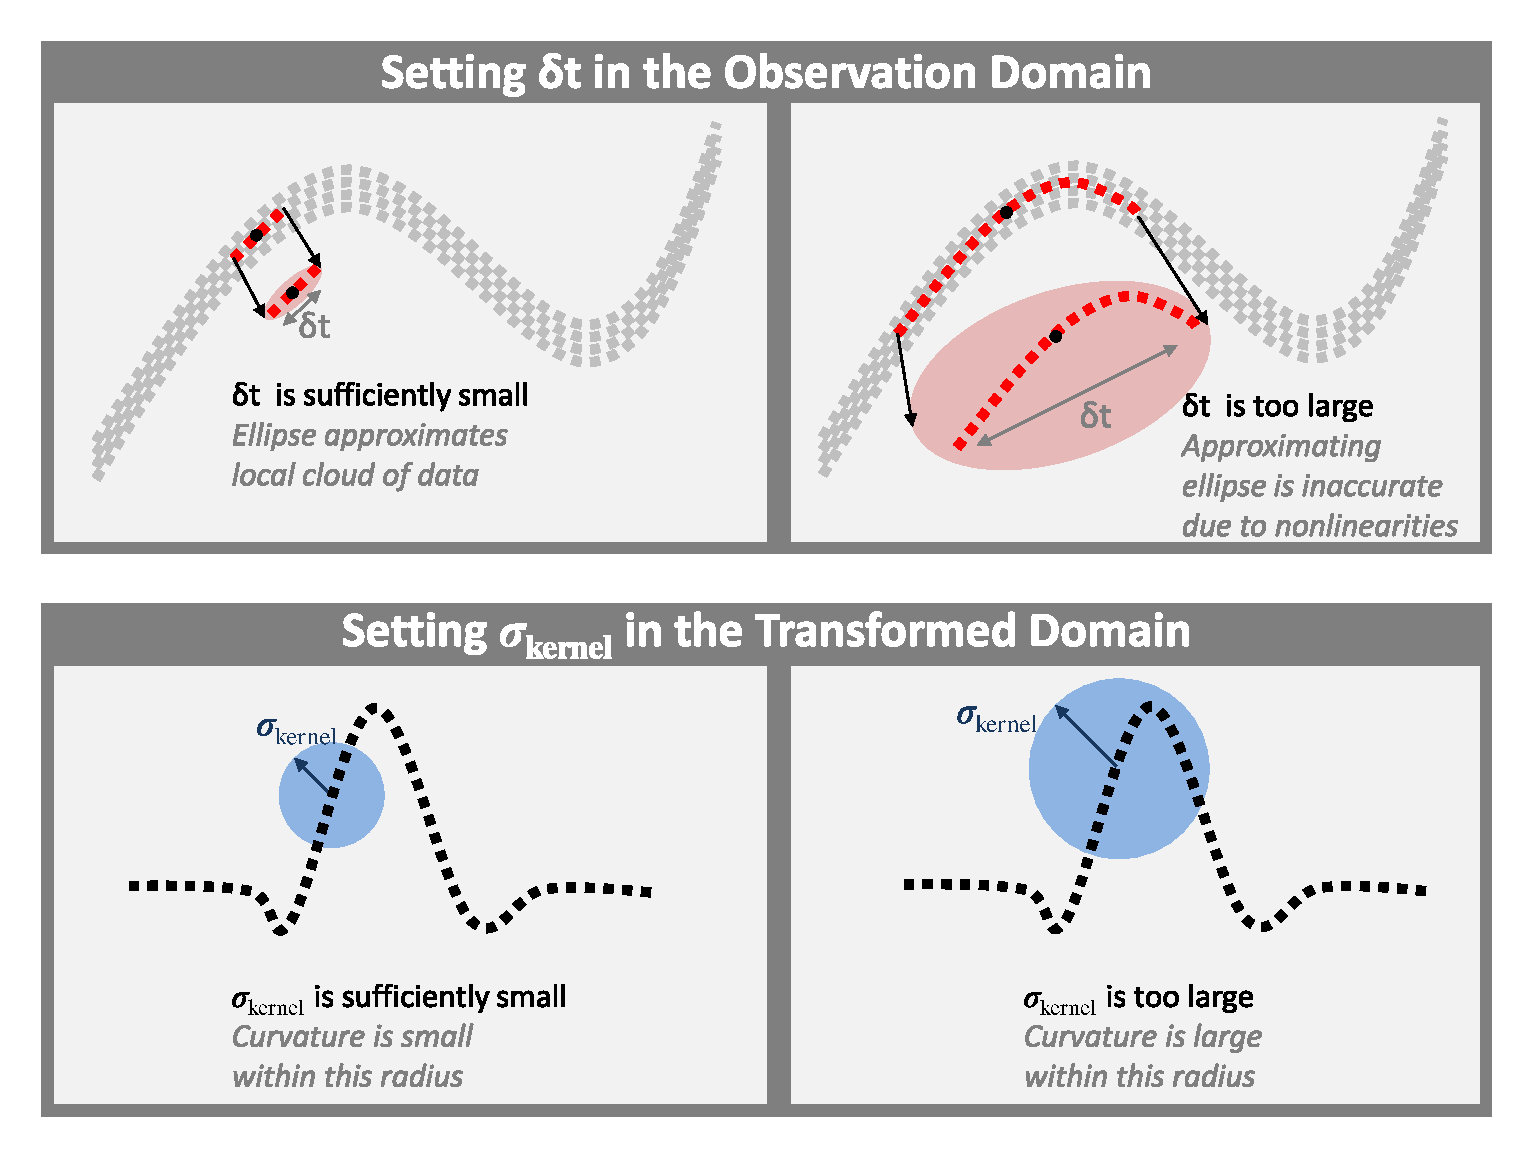
\epsfig{width=\textwidth, file=schematic.eps}
\caption{Illustration of how to choose $\delta t$ and $\sigma_{kernel}$ appropriately. The data shows the evolution of the ``fast'' variable at a fixed value of the ``slow'' variable.  We must choose both parameters so that the curvature effects and other nonlinearities are negligable. }
\label{fig:schematic}
\end{figure}

Our approximation of the pairwise distances will rely on the Taylor expansion of the measurement function $\mathbf{f}$. 
%
We will then {\em empirically} estimate the first-order term in this expansion using simulation bursts to estimate the local covariance.  
%
Accordingly, we will address the accuracy of our method from two standpoints: (1) the accuracy of the Taylor expansion, and (2) the accuracy of the covariance estimation (see Figure~\ref{fig:schematic}).
%
We will present both analytical results for the error bounds, as well as an empirical methodology to set the appropriate parameters for our method to accurately recover the intrinsic slow variable(s). 

%TODO: change ``curvature'' in figure to ``nonlinearity'' in $\sigma_{kernel}$
%TODO: emphasize that if $\delta t$ is too large, then data does not look Gaussian
%TODO: change strip to look different than other data


\subsection{Error analysis of the Mahalanobis distance}

We want to calculate the distance $\|\vec{z}_2 - \vec{z}_1\|$ in terms of the observations $\vec{y} = \mathbf{f}(\vec{x})$. 
%
Let $\mathbf{g} = \mathbf{f}^{-1}: \mathbb{R}^d \mapsto \mathbb{R}^n$, such that
\begin{equation}
\begin{aligned}
g_i(\vec{y}) &=& x_i &=& z_i, & \: 1 \le i \le m \\
\sqrt{\epsilon} g_i(\vec{y}) &=& \sqrt{\epsilon} x_i &=& z_i, & \: m+1 \le i \le n
\end{aligned}
\end{equation}
%
Let $\vec{y}_1 = \mathbf{f}(\vec{x}_1)$, and $\vec{y}_2 = \mathbf{f}(\vec{x}_2)$.
%
%Then, by Taylor expansion, we obtain
%\begin{equation}
%\begin{aligned}
%\xi_{2,i} &=& 
%\xi_{1,i} 
%+ \sum_{j=1}^d \left. \frac{\partial g_i}{\partial y_j} \right|_{Y_1} (y_{2,j} - y_{1,j} ) 
%+ \frac{1}{2} \sum_{j=1}^d \sum_{k=1}^d \left. \frac{\partial^2 g_i}{\partial y_j \partial y_k} \right|_{Y_1} (y_{2,j} - y_{1,j}) (y_{2,k} - y_{1,k}) \\
%&&+ \frac{1}{6} \sum_{j=1}^d \sum_{k=1}^d \sum_{l=1}^d \left. \frac{\partial^3 g_i}{\partial y_j \partial y_k \partial y_l} \right|_{Y_1} (y_{2,j} - y_{1,j}) (y_{2,k} - y_{1,k}) (y_{2,l} - y_{1,l})
%+ \mathcal{O}( \|Y_2 - Y_1\|^4 )
%\end{aligned}
%\end{equation}
%for $1 \le i \le m$, and 
%\begin{equation}
%\begin{aligned}
%\xi_{2,i} &=& 
%\xi_{1,i} 
%+ \sqrt{\epsilon} \left[ \sum_{j=1}^d \left. \frac{\partial g_i}{\partial y_j} \right|_{Y_1} (y_{2,j} - y_{1,j} ) 
%+ \frac{1}{2} \sum_{j=1}^d \sum_{k=1}^d \left. \frac{\partial^2 g_i}{\partial y_j \partial y_k} \right|_{Y_1} (y_{2,j} - y_{1,j}) (y_{2,k} - y_{1,k}) \right. \\
%&& \left.+ \frac{1}{6} \sum_{j=1}^d \sum_{k=1}^d \sum_{l=1}^d \left. \frac{\partial^3 g_i}{\partial y_j \partial y_k \partial y_l} \right|_{Y_1} (y_{2,j} - y_{1,j}) (y_{2,k} - y_{1,k}) (y_{2,l} - y_{1,l}) \right]
%+ \mathcal{O}( \|Y_2 - Y_1\|^4 )
%\end{aligned}
%\end{equation}
%for $m+1 \le i \le n$. 
%
By Taylor expansion of $\mathbf{g}$, we obtain
%
{\small
\begin{equation} \label{eq:distance_taylor_expansion}
\begin{aligned}
&\| \vec{z}_2 - \vec{z}_1 \|^2_2 = \\
& \frac{1}{2} (\vec{y}_2 - \vec{y}_1 )^T \left(\left.(J I_\epsilon J^T)^{-1}\right|_{\vec{y}_1} + \left.( J I_\epsilon J^T)^{-1}\right|_{\vec{y}_2}\right) (\vec{y}_2 - \vec{y}_1 ) \\
& + \frac{1}{2} \sum_{i=1}^m \sum_{jkl=1}^{d} \left( \left. \frac{\partial g_i}{\partial y_j} \right|_{Y_1} \left. \frac{\partial^2 g_i}{\partial y_k \partial y_l} \right|_{Y_1} - \left. \frac{\partial g_i}{\partial y_j} \right|_{Y_2} \left. \frac{\partial^2 g_i}{\partial y_k \partial y_l} \right|_{Y_2} \right) (y_{2,j} - y_{1,j})  (y_{2,k} - y_{1,k})(y_{2,l} - y_{1,l}) \\
& + \frac{\epsilon}{2} \sum_{i=m+1}^n \sum_{jkl=1}^{d} \left( \left. \frac{\partial g_i}{\partial y_j} \right|_{Y_1} \left. \frac{\partial^2 g_i}{\partial y_k \partial y_l} \right|_{Y_1} - \left. \frac{\partial g_i}{\partial y_j} \right|_{Y_2} \left. \frac{\partial^2 g_i}{\partial y_k \partial y_l} \right|_{Y_2} \right) (y_{2,j} - y_{1,j})  (y_{2,k} - y_{1,k})(y_{2,l} - y_{1,l}) \\
& + \frac{1}{8} \sum_{i=1}^m \sum_{jklm=1}^d  \left( \left. \frac{\partial^2 g_i}{\partial y_j \partial y_k} \right|_{Y_1} \left. \frac{\partial^2 g_i}{\partial y_l \partial y_m} \right|_{Y_1} + \left. \frac{\partial^2 g_i}{\partial y_j \partial y_k} \right|_{Y_2} \left. \frac{\partial^2 g_i}{\partial y_l \partial y_m} \right|_{Y_2} \right) (y_{2,j} - y_{1,j})  (y_{2,k} - y_{1,k})(y_{2,l} - y_{1,l})(y_{2,m} - y_{1,m}) \\
& + \frac{\epsilon}{8} \sum_{i=m+1}^n \sum_{jklm=1}^d  \left( \left. \frac{\partial^2 g_i}{\partial y_j \partial y_k} \right|_{Y_1} \left. \frac{\partial^2 g_i}{\partial y_l \partial y_m} \right|_{Y_1} + \left. \frac{\partial^2 g_i}{\partial y_j \partial y_k} \right|_{Y_2} \left. \frac{\partial^2 g_i}{\partial y_l \partial y_m} \right|_{Y_2} \right) (y_{2,j} - y_{1,j})  (y_{2,k} - y_{1,k})(y_{2,l} - y_{1,l})(y_{2,m} - y_{1,m}) \\
& + \frac{1}{6}  \sum_{i=1}^m \sum_{jklm=1}^d  \left( \left. \frac{\partial g_i}{\partial y_j} \right|_{Y_1} \left. \frac{\partial^3 g_i}{ \partial y_k \partial y_l \partial y_m} \right|_{Y_1} + \left. \frac{\partial g_i}{\partial y_j} \right|_{Y_2} \left. \frac{\partial^3 g_i}{ \partial y_k \partial y_l \partial y_m} \right|_{Y_2} \right) (y_{2,j} - y_{1,j})  (y_{2,k} - y_{1,k})(y_{2,l} - y_{1,l})(y_{2,m} - y_{1,m}) \\
& + \frac{\epsilon}{6}  \sum_{i=m+1}^n \sum_{jklm=1}^d  \left( \left. \frac{\partial g_i}{\partial y_j} \right|_{Y_1} \left. \frac{\partial^3 g_i}{ \partial y_k \partial y_l \partial y_m} \right|_{Y_1} + \left. \frac{\partial g_i}{\partial y_j} \right|_{Y_2} \left. \frac{\partial^3 g_i}{ \partial y_k \partial y_l \partial y_m} \right|_{Y_2} \right) (y_{2,j} - y_{1,j})  (y_{2,k} - y_{1,k})(y_{2,l} - y_{1,l})(y_{2,m} - y_{1,m}) \\
& + \mathcal{O} (\|\vec{y}_1 - \vec{y}_2 \|^6 ) 
\end{aligned}
\end{equation}
}
%
where $J$ is the Jacobian of $\mathbf{f}$, and $I_\epsilon$ is a diagonal matrix with $I_{\epsilon,ii} = 1$ for $1 \le i \le m$, and $I_{\epsilon,ii} = \frac{1}{\epsilon}$ for $m+1 \le i \le n$. 

In general, we do not have access to $\mathbf{f}$, $\mathbf{g}$, or any of its derivatives.
%
However, we note that $\left. J I_\epsilon J^T\right|_Y$ is the local covariance of the observed stochastic process at $Y$, which we can empirically estimate from data (this will be discussed in a subsequent section).
%
Therefore, we choose to truncate the distance approximation at the first order term.
%
We call this distance the {\em Mahalanobis distance} \footnote{We would like to note that the Mahalanobis distance is traditionally defined for a fixed covariance matrix. However, following \cite{...}, we will define our Mahalanobis distance locally, using the local covariance at each point.}, 
\begin{equation} \label{eq:mahalanobis_distance}
 \| \vec{y}_2 - \vec{y}_1 \|^2_M = \frac{1}{2} (\vec{y}_2 - \vec{y}_1 )^T \left(\left.(J I_\epsilon J^T)^{-1}\right|_{\vec{y}_1} + \left.(J I_\epsilon J^T)^{-1}\right|_{\vec{y}_2}\right) (\vec{y}_2 - \vec{y}_1 )
\end{equation}
%
and we define the error incurred by using the Mahalanobis distance to approximate the true distance between the points as
\begin{equation} \label{eq:mahanaobis_error}
e_M(\vec{y}_1, \vec{y}_2) \equiv \| \vec{z}_2 - \vec{z}_1 \|^2_2 - \| \vec{y}_2 - \vec{y}_1 \|^2_M 
\end{equation}

%We can bound the error by
%\begin{equation}
%| e_M(Y_1, Y_2)  | \le n \left( \left| K_1 K_2 \right| + \left| \frac{ K_2^2}{4} \right|  + \left| \frac{K_1 K_3}{3} \right|  \right) \| Y_2 - Y_1 \| ^4  
%+ \mathcal{O} (\|Y_1 - Y_2 \|^6 ) 
%\end{equation}
%%
%where
%%
%\begin{equation}
%\begin{aligned}
%K_1 &= \sup_{i,j,Y} |g_j^i(Y)|\\
%K_2 &= \sup_{i,j,k,Y} |g_{jk}^i(Y)|\\
%K_3 &= \sup_{i,j,k,l,Y} |g_{jkl}^i(Y)|
%\end{aligned}
%\end{equation}



\subsection{Error analysis of the covariance estimation}

To compute the Mahalanobis distance in \eqref{eq:mahalanobis_distance}, we require $J I_\epsilon J^T$. 
%
From \cite{...}, we know that $J I_\epsilon J^T = C$, where $C$ is the local covariance of the observed stochastic process. 
%
Therefore, we would like to estimate the local covariance at a point $\vec{x}_t$. 

We know that, for a stochastic process following \eqref{eq:general_SDE} and observed through a function $\mathbf{f}$, the covariance $C$ is given by 
\begin{equation}
C_{jk}(\vec{x}_t) = 
\sum_{i=1}^m \left. \frac{\partial f_j}{\partial x_i} \right|_{\vec{x}_t} \left. \frac{\partial f_k}{\partial x_i} \right|_{\vec{x}_t} 
+ \frac{1}{\epsilon} \sum_{i=m+1}^n \left. \frac{\partial f_j}{\partial x_i} \right|_{\vec{x}_t} \left. \frac{\partial f_k}{\partial x_i} \right|_{\vec{x}_t} 
\end{equation}

We will use local simulation bursts to estimate the local covariance.
%
Let $\vec{x}_{t + \delta t}$ denote samples at time $t + \delta t> t$. 
%
For the general SDE formulation outlined in \eqref{eq:general_SDE}, the estimated covariance $\hat{C}$ is \cite{...} as
\begin{equation} \label{eq:estimated_cov}
\begin{aligned}
\hat{C}_{jk} (\vec{x}_t, \delta t) = & 
\frac{1}{\delta t} \left(  \mathbb{E} \left[ f_j(\vec{x}_{t+\delta t}) f_k(\vec{x}_{t+\delta t}) \right] - \mathbb{E}[f_j(\vec{x}_{t+\delta t})]\mathbb{E}[f_k(\vec{x}_{t+\delta t})]   \right)\\
= & \sum_{i=1}^m \left. \frac{\partial f_j}{\partial x_i} \right|_{\vec{x}_t} \left. \frac{\partial f_k}{\partial x_i} \right|_{\vec{x}_t}  
 + \frac{1}{\epsilon} \sum_{i=m+1}^n \left. \frac{\partial f_j}{\partial x_i} \right|_{\vec{x}_t} \left. \frac{\partial f_k}{\partial x_i} \right|_{\vec{x}_t} \\
& + \frac{1}{\delta t} \sum_{i=1}^m \left. \frac{\partial f_j}{\partial x_i} \right|_{\vec{x}_t} \mathbb{E} \left[ \left( \int_t^\tau dW_s^i  \right) \left( \int_t^{t + \delta t} \int_t^{s_2} \frac{\partial^2 f_k}{\partial x_i^2} dW_{s_1}^i dW_{s_2}^i  \right) \right] \\
& + \frac{1}{\epsilon^{3/2} \delta t} \sum_{i=m+1}^n \left. \frac{\partial f_j}{\partial x_i} \right|_{\vec{x}_t} \mathbb{E} \left[ \left( \int_t^{t + \delta t} dW_s^i  \right) \left( \int_t^{t + \delta t} \int_t^{s_2} \frac{\partial^2 f_k}{\partial x_i^2} dW_{s_1}^i dW_{s_2}^i  \right) \right] \\
& + \frac{1}{\delta t} \sum_{i=1}^m \left. \frac{\partial f_k}{\partial x_i} \right|_{\vec{x}_t}  \mathbb{E} \left[ \left( \int_t^{t + \delta t} dW_s^i \right)  \left( \int_t^{t + \delta t} \int_t^{s_2} \frac{\partial^2 f_j}{\partial x_i^2}  dW_{s_1}^i dW_{s_2}^i \right) \right] \\
& + \frac{1}{\epsilon^{3/2} \delta t} \sum_{i=m+1}^n \left. \frac{\partial f_k}{\partial x_i} \right|_{\vec{x}_t}  \mathbb{E} \left[ \left( \int_t^{t + \delta t} dW_s^i \right)  \left( \int_t^{t + \delta t} \int_t^{s_2} \frac{\partial^2 f_j}{\partial x_i^2}  dW_{s_1}^i dW_{s_2}^i \right) \right] \\
&+ \mathcal{O} (\delta t) 
\end{aligned}
\end{equation}
%
However, for the specific case when $\mathbf{f}$ is linear, the $\mathcal{O}(\sqrt{\delta t})$ drop out, and we must consider higher-order terms. 
%
In this case, 
%
{\small 
\begin{equation} \label{eq:estimated_cov_linear_f}
\begin{aligned}
\hat{C}_{jk} (\vec{x}_t, \delta t) = & 
\frac{1}{\delta t} \left(  \mathbb{E} \left[ f_j(\vec{x}_{t + \delta t}) f_k(\vec{x}_{t + \delta t}) \right] - \mathbb{E}[f_j(\vec{x}_{t + \delta t})]\mathbb{E}[f_k(\vec{x}_{t + \delta t})]   \right)\\
= & \sum_{i=1}^m \left. \frac{\partial f_j}{\partial x_i} \right|_{\vec{x}_t} \left. \frac{\partial f_k}{\partial x_i} \right|_{\vec{x}_t}  
 + \frac{1}{\epsilon} \sum_{i=m+1}^n \left. \frac{\partial f_j}{\partial x_i} \right|_{\vec{x}_t} \left. \frac{\partial f_k}{\partial x_i} \right|_{\vec{x}_t} \\
 & + \frac{1}{\delta t} \sum_{i=1}^m \left. \frac{\partial f_j}{\partial x_i} \right|_{\vec{x}_t}  \mathbb{E} \left[ \left(\int_t^{t + \delta t} dW_s^i \right)  \left(\int_t^{t + \delta t} \int_{t}^{s_2} \left(  \sum_{l=1}^m \frac{\partial a_l}{\partial x_i} \frac{\partial f_k}{\partial x_l}  + \frac{1}{\epsilon} \sum_{l=m+1}^m \frac{\partial a_l}{\partial x_i} \frac{\partial f_k}{\partial x_l} \right)  dW_{s_1}^i ds_2 \right) \right] \\ 
 & + \frac{1}{\epsilon \delta t} \sum_{i=m+1}^n \left. \frac{\partial f_j}{\partial x_i} \right|_{\vec{x}_t}  \mathbb{E} \left[ \left(\int_t^{t + \delta t} dW_s^i \right)  \left(\int_t^{t + \delta t} \int_{t}^{s_2} \left(  \sum_{l=1}^m \frac{\partial a_l}{\partial x_i} \frac{\partial f_k}{\partial x_l}  + \frac{1}{\epsilon} \sum_{l=m+1}^m \frac{\partial a_l }{\partial x_i} \frac{\partial f_k}{\partial x_l} \right)  dW_{s_1}^i ds_2 \right) \right] \\ 
 & + \frac{1}{\delta t} \sum_{i=1}^m  \left. \frac{\partial f_k}{\partial x_i} \right|_{\vec{x}_t}  \mathbb{E} \left[ \left(\int_t^{t + \delta t} dW_s^i \right)  \left(\int_t^{t + \delta t} \int_{t}^{s_2} \left(  \sum_{l=1}^m \frac{\partial a_l}{\partial x_i} \frac{\partial f_j}{\partial x_l}  + \frac{1}{\epsilon} \sum_{l=m+1}^m \frac{\partial a_l }{\partial x_i} \frac{\partial f_j}{\partial x_l} \right) dW_{s_1}^i ds_2 \right) \right] \\
& + \frac{1}{\epsilon \delta t} \sum_{i=m+1}^n  \left. \frac{\partial f_k}{\partial x_i} \right|_{\vec{x}_t}  \mathbb{E} \left[ \left(\int_t^{t + \delta t} dW_s^i \right)  \left(\int_t^{t + \delta t} \int_{t}^{s_2} \left(  \sum_{l=1}^m \frac{\partial a_l}{\partial x_i} \frac{\partial f_j}{\partial x_l}  + \frac{1}{\epsilon} \sum_{l=m+1}^m \frac{\partial a_l }{\partial x_i} \frac{\partial f_j}{\partial x_l} \right) dW_{s_1}^i ds_2 \right) \right] \\
& + \mathcal{O} (\delta t^{3/2})
 \end{aligned}
\end{equation}
}
%
For both cases, we define the error in the covariance estimation as
%
\begin{equation} \label{eq:cov_error}
\begin{aligned}
e_C (\vec{x}_t, \delta t) \equiv \hat{C} (\vec{x}_t, \delta t)  - C(\vec{x}_t) 
\end{aligned}
\end{equation}

\section{Empirical Estimation of Parameters}

TODO: explain more

We would like to empirically set the simulation and analysis parameters so that we can accurately recover the slow variables from data. 
%
There are two parameters: $\sigma_{kernel}$, the diffusion maps kernel scale, and $\tau - t$, the timescale of the ``burst'' used to estimate the covariance. 

$\sigma_{kernel}$ controls which distances we ``trust''.
%
Therefore, we want the Mahalanobis distance approximation to be accurate within a ball of radius $\sigma_{kernel}$. 
%
From \eqref{eq:distance_taylor_expansion}, we can see that, for $e_M$ to be small, we want $\|Y_2 - Y_1 \|^2_M$ to vary quadratically with $\|Y_2 - Y_1\|_2$.

From \eqref{eq:estimated_cov} and \eqref{eq:estimated_cov_linear_f}, for $e_C$ to be accurate, we want $\hat{C}$ to be constant with $\delta t$. 

We can use simulations to check both of these conditions empirically. 

\section{Results}

For illustrative purposes, we will consider the following two-dimensional SDE as a specific example of \eqref{eq:general_SDE}. 
\begin{equation} \label{eq:specific_SDE}
\begin{aligned}
dx_1 &=& adt &+& dW_1\\
dx_2 &=& -\frac{x_2}{\epsilon} dt &+& \frac{1}{\sqrt{\epsilon}} dW_2
\end{aligned}
\end{equation}
%
where $a$ is a constant of order 1 (we will take $a=3$). 
%
So $x_1$ is the slow variable, and $x_2$ is a fast noise whose equilibrium measure is bounded and $\mathcal{O}(1)$.
%
Figure~\ref{fig:initial_data} shows data simulated from this SDE, colored by time.
%
We would like to recover $x_1$ (the slow variable) using data-driven techniques.

\begin{figure}[h]
\centering
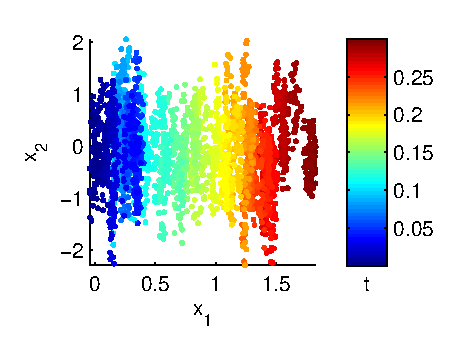
\epsfig{width=0.5\textwidth, file=data_init.eps}
\caption{The original data, simulated from \eqref{eq:specific_SDE} with $\epsilon = 10^{-3}$. We take $3000$ timesteps with $dt = 10^{-4}$. The data is colored by time. }
\label{fig:initial_data}
\end{figure}

\subsection{Linear functions}

In the first example, our transformation $\mathbf{f}$ will be the identity function so that the fast and slow remain uncoupled,
\begin{equation}
\mathbf{f}(\vec{x}) = \begin{bmatrix} x_1 \\ x_2 \end{bmatrix}
\end{equation}
%
\begin{equation}
\mathbf{g}(\vec{y}) = \mathbf{f}^{-1} (\vec{y}) = \begin{bmatrix} y_1 \\ y_2 \end{bmatrix}
\end{equation}

In this case, $e_M = 0$, as the second- and higher-order derivatives of $\mathbf{g}$ are all 0. 

For this example, the analytical covariance is
 \begin{equation}
C(\vec{x}_t) = 
\begin{bmatrix}
1 & 0 \\
0 & \frac{1}{\epsilon}
\end{bmatrix}
\end{equation}

\subsubsection{NIVs versus DMAPS}

We first want to demonstrate the utility of NIVs over DMAPS. 
%
We compute the first (nontrivial) NIV and DMAPS coordinate using the data in Figure~\ref{fig:initial_data}. 
%
The results are shown in Figure~\ref{fig:NIV_versus_DMAPS}.
%
NIV accurately recovers the slow variable (the coloring in Figure~\ref{fig:NIV_versus_DMAPS}(a) is consistent with the coloring in Figure~\ref{fig:initial_data}). 
%
In contrast, DMAPS does not recover the slow variable. 

\begin{figure}[t]
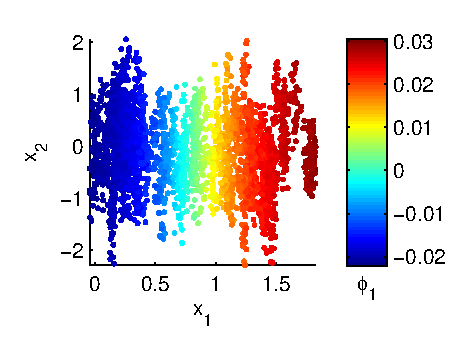
\epsfig{width=0.5\textwidth, file=data_linear_NIV.eps}
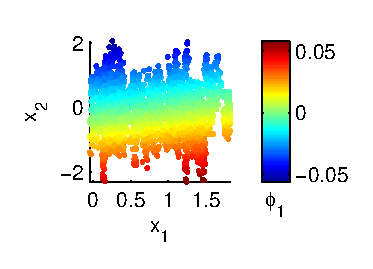
\epsfig{width=0.5\textwidth, file=data_linear_DMAPS.eps}
\caption{(a) The data from Figure~\ref{fig:initial_data}, colored by the first NIV. (b) The data from Figure~\ref{fig:initial_data}, colored by the first DMAPS variable. Note that we do {\em not} recover the slow variable.}
\label{fig:NIV_versus_DMAPS}
\end{figure}

\subsubsection{Errors in covariance estimation}

From \eqref{eq:estimated_cov_linear_f}, we find that 
\begin{equation}
\begin{aligned}
e_{C, 11}(\vec{x}_t, \delta t) &= 
e_{C, 12}(\vec{x}_t, \delta t) = 
e_{C, 21}(\vec{x}_t, \delta t) = 0 \\
e_{C, 22}(\vec{x}_t, \delta t) &= 
\frac{-2}{\epsilon^2 \delta t} \mathbb{E} \left[ \left(\int_t^{t + \delta t} dW_s^2 \right)  \left(\int_t^{t + \delta t} \int_{t}^{s_2} -dW_{s_1}^2 ds_2 \right) \right]  
+ \mathcal{O} (\delta t^{3/2})
\end{aligned}
\end{equation}
%
Therefore, $\|e_C \| = \mathcal{O}\left(\frac{\delta t}{\epsilon^2} \right)$ and so we need to choose $\delta t < \epsilon^2$ so that the covariance estimation is accurate. 
%
To empirically find this regime, we can plot $\|\hat{C}\|$ as a function of $\delta t$. 
%
We know 
\begin{equation}
\hat{C}(\vec{x}_t, \delta t) = C(\vec{x}_t) + e_C(\vec{x}_t, \delta t) = C(\vec{x}_t) + \mathcal{O}\left(\frac{\delta t}{\epsilon^2} \right)
\end{equation} 
%
Therefore, when $e_C$ is small, $\hat{C}$ will be constant as a function of $\delta t$, and when $e_C$ is large, $\hat{C}$ will be linear in $\delta t$.
%
This is shown in Figure~\ref{fig:cov_error}, and we can see (both analytically and empirically)
$\delta t < 10^{-5}$ corresponds to the constant regime.

\begin{figure}[t]
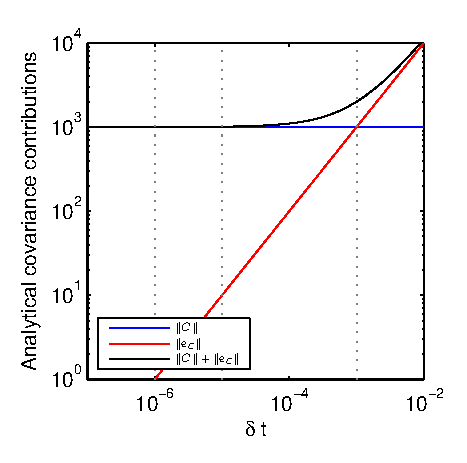
\epsfig{width=0.5\textwidth, file=C_dt_analytical_linear.eps}
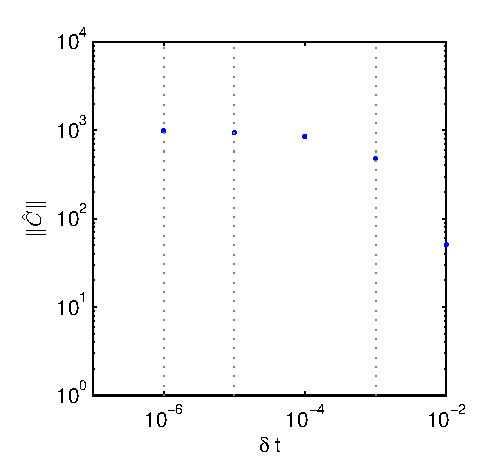
\epsfig{width=0.5\textwidth, file=C_dt_linear.eps}
%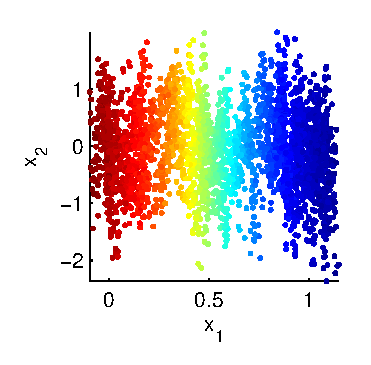
\epsfig{width=0.5\textwidth, file=data_linear_NIV_smalldt.eps}
\caption{(a) The analytical expressions for the contibutions to the covariance as a function of the time burst. (b) The average estimated covariance $\| \hat{C} \|$ as a function of the time burst $\delta t$. }
\label{fig:cov_error}
\end{figure}

\subsubsection{Recovery of Fast Variable}


Note that, for this linear example, $e_C$ is a diagonal matrix. 
%
Therefore, taking $\delta t$ ``too large'' will not lead to mixing of the fast/slow variables, or nonlinear effects, but rather, only affect the ''perceived'' timescales of the fast/slow. 
%
When the time scale of the burst is smaller than that of the equilibration time of the fast variable, the estimated covariance is constant and the fast variable is collapsed significantly relative to the slow variable.
%
This means that the fast variable is recovered {\em very} far down in the DMAPS eigenvectors.
%
However, if the time scale of the burst is {\em longer} than the saturation time of the fast variable, the estimated covariance changes: the variance in the slow direction continues to grow, while the variance in the fast direction is fixed.
%
This means that the collapse of the fast variable is less pronounced relative to the slow variable, and the fast variable is recovered in a higher eigenvector. 

\begin{figure}[t]
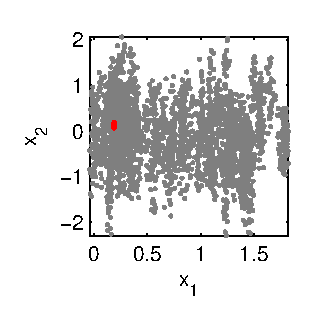
\epsfig{width=0.3\textwidth, file=data_linear_burst1.eps}
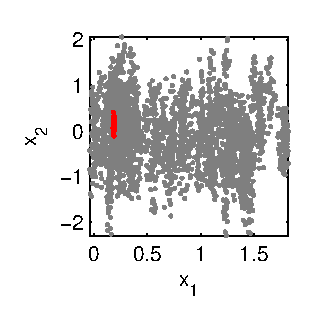
\epsfig{width=0.3\textwidth, file=data_linear_burst2.eps}
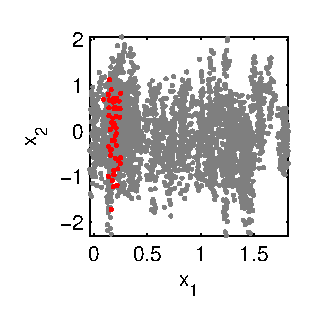
\epsfig{width=0.3\textwidth, file=data_linear_burst3.eps}

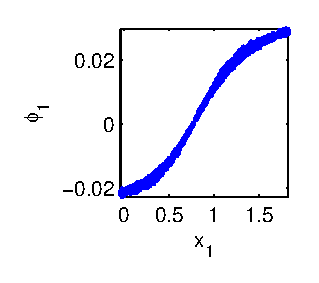
\epsfig{width=0.3\textwidth, file=data_linear_slow1.eps}
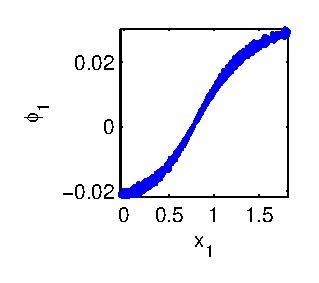
\epsfig{width=0.3\textwidth, file=data_linear_slow2.eps}
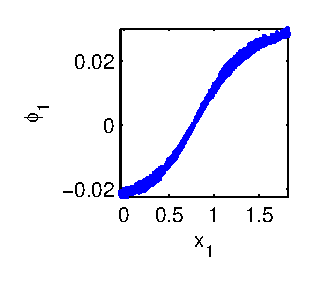
\epsfig{width=0.3\textwidth, file=data_linear_slow3.eps}

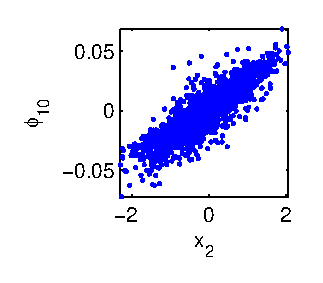
\epsfig{width=0.3\textwidth, file=data_linear_fast1.eps}
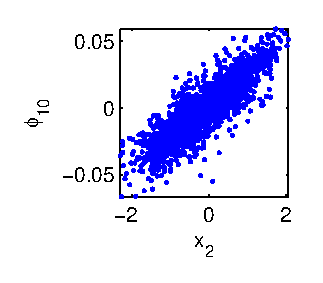
\epsfig{width=0.3\textwidth, file=data_linear_fast2.eps}
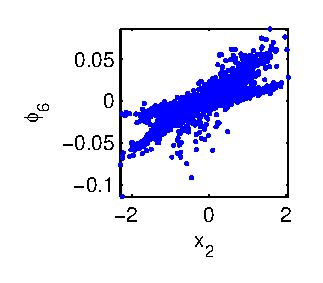
\epsfig{width=0.3\textwidth, file=data_linear_fast3.eps}

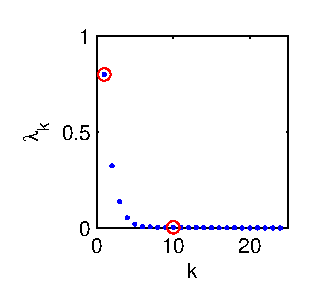
\epsfig{width=0.3\textwidth, file=data_linear_evals1.eps}
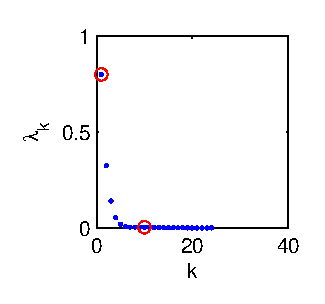
\epsfig{width=0.3\textwidth, file=data_linear_evals2.eps}
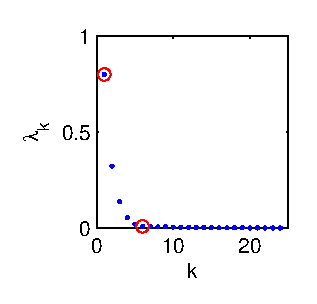
\epsfig{width=0.3\textwidth, file=data_linear_evals3.eps}

\caption{Correlation between dmaps coordinate and fast variable for $\delta t = 10^{-9}, 10^{-6},$ and $10^{-3}$. }
\label{fig:recover_fast}
\end{figure}

\subsection{Nonlinear functions}

In the second example, our data will be warped into half-moon shapes
\begin{equation} \label{eq:nonlinear_function}
\mathbf{f}(\vec{x}) = 
\begin{bmatrix} 
x_1 + x_2^2 \\
x_2
\end{bmatrix}
\end{equation}

\begin{equation}
\mathbf{g}(\vec{y}) = \mathbf{f}^{-1} (\vec{y}) = \begin{bmatrix} y_1 - y_2^2 \\ y_2 \end{bmatrix}
\end{equation}

For this example, the analytical covariance is 
\begin{equation}
C(\vec{x}) = \begin{bmatrix}
1+ \frac{4 x_2^2}{\epsilon} & \frac{2 x_2}{\epsilon} \\
\frac{2 x_2}{\epsilon} & \frac{1}{\epsilon} 
\end{bmatrix}
\end{equation}

\begin{equation}
C^{-1}(\vec{x}) = 
\epsilon
\begin{bmatrix}
\frac{1}{\epsilon} & -\frac{2 x_2}{\epsilon} \\
-\frac{2 x_2}{\epsilon} & 1+ \frac{4 x_2^2}{\epsilon}
\end{bmatrix} = 
\begin{bmatrix}
1 & -2 x_2 \\
-2 x_2 & \epsilon+ 4 x_2^2
\end{bmatrix} 
\end{equation}

\begin{figure}[t]
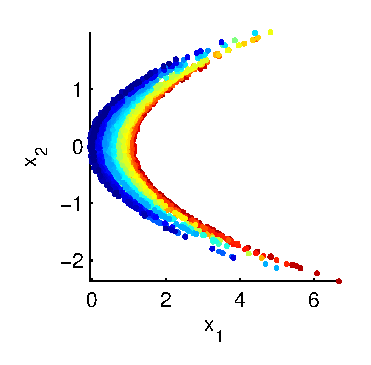
\epsfig{width=0.3\textwidth, file=data_init_nonlinear.eps}
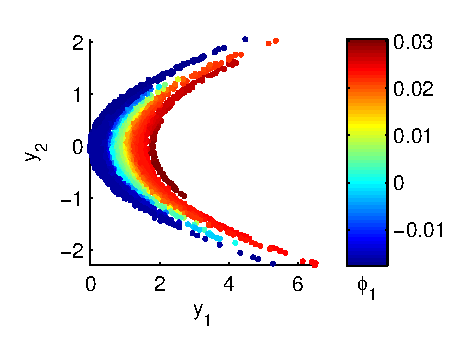
\epsfig{width=0.3\textwidth, file=data_nonlinear_NIV.eps}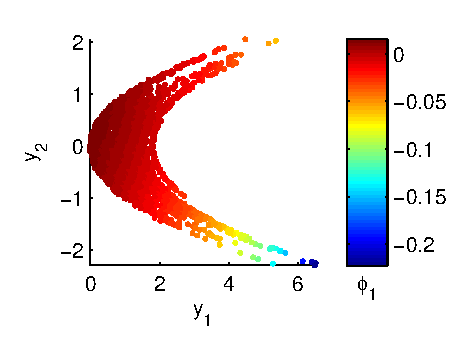
\epsfig{width=0.3\textwidth, file=data_nonlinear_DMAPS.eps}\caption{(a) The data, simulated from \eqref{eq:specific_SDE} and transformed by $\mathbf{f}$,  with $\epsilon = 10^{-3}$. We take $3000$ timesteps with $dt = 10^{-4}$. (b) The data from (a), colored by the first NIV. (c) The data from (a), colored by the first DM variable.}
\label{fig:initial_data_nonlinear}
\end{figure}


\subsubsection{Errors in Mahalanobis distance}

From \eqref{eq:distance_taylor_expansion}, we have 
\begin{equation}
e_M(\vec{y}_1, \vec{y}_2) = 3 (y_{2,2} - y_{1,2})^4 
+ \mathcal{O} (\|\vec{y}_1 - \vec{y}_2 \|^6 ) 
\end{equation}
%
Therefore, $\|e_M \| = \mathcal{O}\left(\| \vec{y}_2 - \vec{y}_1\|^4 \right)$
%
We know 
\begin{equation}
\begin{aligned}
\| \vec{z}_2 - \vec{z}_1 \|^2_2 
& = \| \vec{y}_2 - \vec{y}_1 \|_M^2 + e_M(\vec{y}_1, \vec{y}_2) \\
& = \frac{1}{2} (\vec{y}_2 - \vec{y}_1 )^T \left(\left.(J I_\epsilon J^T)^{-1}\right|_{\vec{y}_1} + \left.(J I_\epsilon J^T)^{-1}\right|_{\vec{y}_2}\right) (\vec{y}_2 - \vec{y}_1 ) 
+ \mathcal{O} (\|\vec{y}_1 - \vec{y}_2 \|^4 ) 
\end{aligned}
\end{equation} 
%
Therefore, when $e_M$ is small, $\|\vec{y}_2 - \vec{y}_1 \|_M^2$ will vary quadratically as a function of $\|\vec{y}_1 - \vec{y}_2 \|_2$.
%
To empirically find this regime, we can plot $\|\vec{y}_2 - \vec{y}_1 \|_M^2$ as a function of $\|\vec{y}_1 - \vec{y}_2 \|_2$. 
%
This is shown in Figure~\ref{fig:initial_data_nonlinear}, and we can see (both analytically and empirically)
$\|\vec{y}_2 - \vec{y}_1 \|^2_M < 1$ corresponds to the quadratic regime.
%
We therefore want to choose $\sigma_{kernel} < 1$ in the diffusion maps calculation so that we only consider pairwise distances where $e_M$ is small.

\subsubsection{Errors in covariance estimation}

From \eqref{eq:estimated_cov}, we find that
\begin{equation}
\begin{aligned}
 e_{C,11}(\vec{x}_t, \delta t) =& \frac{4}{\epsilon^{3/2} \delta t} x_{t,2} \mathbb{E} \left[ \left( \int_t^{t + \delta t} dW_s^2  \right) \left( \int_t^{t + \delta t} \int_t^{s_2} dW_{s_1}^2 dW_{s_2}^2  \right) \right] 
+ \mathcal{O} (\delta t) \\
e_{C,12}(\vec{x}_t, \delta t) =
e_{C,21}(\vec{x}_t, \delta t)  =&
\frac{2}{\epsilon^{3/2} \delta t}  \mathbb{E} \left[ \left( \int_t^{t + \delta t} dW_s^2 \right)  \left( \int_t^\tau \int_t^{s_2}  dW_{s_1}^2 dW_{s_2}^2 \right) \right] 
+ \mathcal{O} (\delta t) \\
 e_{C,22}(\vec{x}_t, \delta t) =& \mathcal{O} (\delta t) 
\end{aligned}
\end{equation}
%
Again, we plot $\| \hat{C} \|$ as a function of $\delta t$, and look for the constant regime, which indicates where $e_C$ is small.
%
This is shown in Figure~\ref{fig:initial_data_nonlinear}. 

\begin{figure}[h]
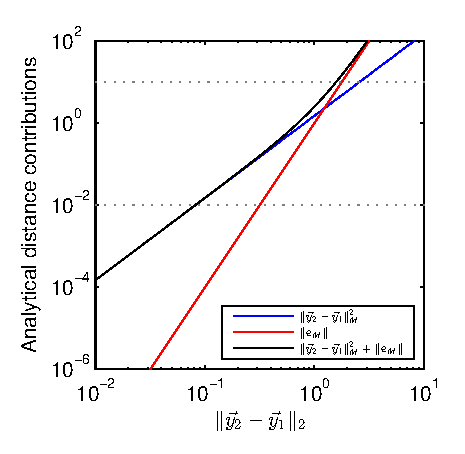
\epsfig{width=0.4\textwidth, file=dist_dy_analytical_nonlinear.eps}
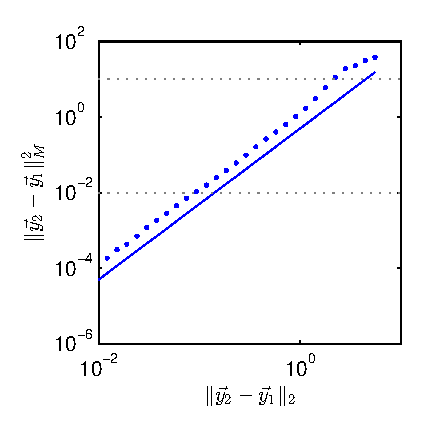
\epsfig{width=0.4\textwidth, file=dist_dy_nonlinear.eps}

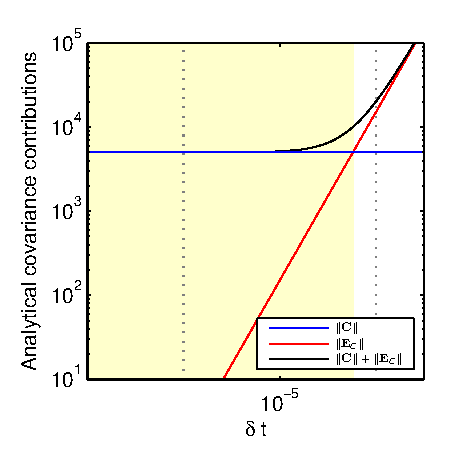
\epsfig{width=0.4\textwidth, file=C_dt_analytical_nonlinear.eps}
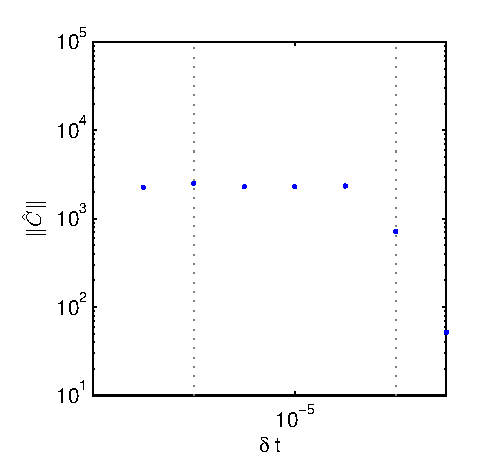
\epsfig{width=0.4\textwidth, file=C_dt_nonlinear.eps}

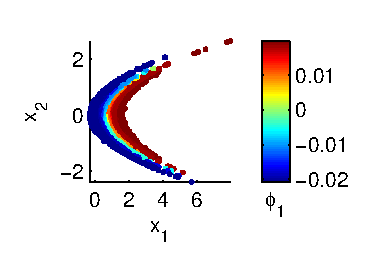
\epsfig{width=0.3\textwidth, file=data_nonlinear_NIV_good.eps}
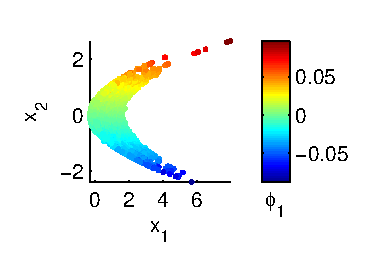
\epsfig{width=0.3\textwidth, file=data_nonlinear_NIV_bad_kernel.eps}
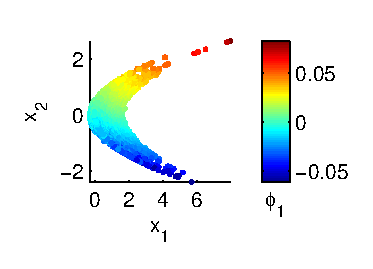
\epsfig{width=0.3\textwidth, file=data_nonlinear_NIV_bad_dt.eps}

\caption{(a) The analytical expressions for the contributions to the distance approximation as a function of $\| \vec{y}_2 - \vec{y}_1\|_2$. (b) The average estimated Mahalanobis distance $\| \vec{y}_2 - \vec{y}_1\|^2_M$ as a function of the distance $\| \vec{y}_2 - \vec{y}_1\|_2$. (c) The analytical expressions for the contibutions to the covariance as a function of the time burst. (d) The average estimated covariance $\| \hat{C} \|$ as a function of the time burst $\delta t$. (e) Data, colored by the first NIV, when $\sigma_{kernel}$ and $\delta t$ are chosen appropriately. (f) Data, colored by the first NIV, when $\sigma_{kernel}$  is too large.  (e) Data, colored by the first NIV, when $\delta t$ is too large. }
\label{fig:cov_error_nonlinear}
\end{figure}

\section{Conclusion}

We showed that in certain cases (when we do {\em not} have a simulator where we can change $\delta t$), the data cannot be processed as-is (we cannot find the right kernel scale given a fixed $\delta t$ such that we can accurately recover the slow variable). 

If the cloud of samples is too big then we can observe the cloud of clouds (and those clouds can be histograms, Fourier, scattering, etc.) as a way to get smaller clouds. 


Richardson extrapolation could allow us to get an estimate of a second-order term in the covariance estimation, thereby locally approximating the function using a quadratic form, rather than a linear form,  which can lead to a better/improved/more accurate ``Mahalanobis'' metric. 


%\appendix
%
%\section{Error in the Mahalanobis distance}
%
%In this section $g_j^i = \frac{\partial g_i}{\partial y_j}$. 
%%
%Also, this algebra does {\em not} include the contributions from the multiscale scaling $\epsilon$. 
%
%By Taylor expansion around $Y_1$, we have
%%
%\begin{equation}
%\begin{aligned}
%X_2^i &=& X_1^i + \sum_j g_j^i (Y_1) (Y^j_2 - Y^j_1 ) 
%+ \frac{1}{2} \sum_{kl}  g^i_{kl} (Y_1) (Y^k_2 - Y^k_1)(Y^l_2 - Y^l_1) \\
%&&+ \frac{1}{6} \sum_{klm}  g^i_{klm} (Y_1) (Y^k_2 - Y^k_1)(Y^l_2 - Y^l_1) (Y^m_2 - Y^m_1) 
%+ \mathcal{O}( \|Y_2 - Y_1\|^4 )
%\end{aligned}
%\end{equation}
%%
%Then computing the distance,
%%
%\begin{equation}
%\begin{aligned}
%&&\| X_2 - X_1 \|^2 \\
%&=&  \sum_i (X_2^i - X_1^i)^2 \\
%&=& \sum_i  \left( \sum_j g_j^i (Y_1) (Y^j_2 - Y^j_1 )  \right.
%+ \frac{1}{2} \sum_{kl}  g^i_{kl} (Y_1) (Y^k_2 - Y^k_1)(Y^l_2 - Y^l_1) \\
%&&+ \left.  \frac{1}{6} \sum_{klm}  g^i_{klm} (Y_1) (Y^k_2 - Y^k_1)(Y^l_2 - Y^l_1) (Y^m_2 - Y^m_1) 
% + \mathcal{O}( \|Y_2 - Y_1\|^4 ) \right)^2 \\
%&=& \sum_{ijk} g_j^i (Y_1) g_k^i (Y_1) (Y^j_2 - Y^j_1 ) (Y^k_2 - Y^k_1 ) \\
%&& + \sum_{ijkl} g_j^i (Y_1) g^i_{kl} (Y_1) (Y^j_2 - Y^j_1 )  (Y^k_2 - Y^k_1)(Y^l_2 - Y^l_1) \\
%&& + \frac{1}{4} \sum_{ijklm}  g^i_{jk} (Y_1) g^i_{lm} (Y_1) (Y^j_2 - Y^j_1) (Y^k_2 - Y^k_1) (Y^l_2 - Y^l_1) (Y^m_2 - Y^m_1) \\
%&& + \frac{1}{3} \sum_{ijklm}  g^i_{j} (Y_1) g^i_{klm} (Y_1) (Y^j_2 - Y^j_1) (Y^k_2 - Y^k_1) (Y^l_2 - Y^l_1) (Y^m_2 - Y^m_1) \\
%&& + \mathcal{O} (\|Y_1 - Y_2 \|^5 )
%\end{aligned}
%\end{equation}
%%
%Expanding around $X_2$ yields
%%
%\begin{equation}
%\begin{aligned}
%&&\| X_2 - X_1 \|^2 \\
%&=&  \sum_i (X_2^i - X_1^i)^2 \\
%&=& \sum_{ijk} g_j^i (Y_2) g_k^i (Y_2) (Y^j_2 - Y^j_1 ) (Y^k_2 - Y^k_1 ) \\
%&& - \sum_{ijkl} g_j^i (Y_2) g^i_{kl} (Y_2) (Y^j_2 - Y^j_1 )  (Y^k_2 - Y^k_1)(Y^l_2 - Y^l_1) \\
%&& + \frac{1}{4} \sum_{ijklm}  g^i_{jk} (Y_2) g^i_{lm} (Y_2) (Y^j_2 - Y^j_1) (Y^k_2 - Y^k_1) (Y^l_2 - Y^l_1) (Y^m_2 - Y^m_1) \\
%&& + \frac{1}{3} \sum_{ijklm}  g^i_{j} (Y_2) g^i_{klm} (Y_2) (Y^j_2 - Y^j_1) (Y^k_2 - Y^k_1) (Y^l_2 - Y^l_1) (Y^m_2 - Y^m_1) \\
%&& + \mathcal{O} (\|Y_1 - Y_2 \|^5 )
%\end{aligned}
%\end{equation}
%%
%Averaging the two expansions yields
%%
%\begin{equation}
%\begin{aligned}
%&&\| X_2 - X_1 \|^2 \\
%&=&  \sum_i (X_2^i - X_1^i)^2 \\
%&=& \frac{1}{2} \sum_{ijk} \left( g_j^i (Y_1) g_k^i (Y_1) + g_j^i (Y_2) g_k^i (Y_2) \right) (Y^j_2 - Y^j_1 ) (Y^k_2 - Y^k_1 ) \\
%&& + \frac{1}{2} \sum_{ijkl} \left( g_j^i (Y_1) g^i_{kl} (Y_1) - g_j^i (Y_2) g^i_{kl} (Y_2) \right) (Y^j_2 - Y^j_1 )  (Y^k_2 - Y^k_1)(Y^l_2 - Y^l_1) \\
%&& + \frac{1}{8} \sum_{ijklm}  \left( g^i_{jk} (Y_1) g^i_{lm} (Y_1) + g^i_{jk} (Y_2) g^i_{lm} (Y_2)  \right) (Y^j_2 - Y^j_1) (Y^k_2 - Y^k_1) (Y^l_2 - Y^l_1) (Y^m_2 - Y^m_1) \\
%&& + \frac{1}{6} \sum_{ijklm}  \left( g^i_{j} (Y_1) g^i_{klm} (Y_1) + g^i_{j} (Y_2) g^i_{klm} (Y_2)  \right)(Y^j_2 - Y^j_1) (Y^k_2 - Y^k_1) (Y^l_2 - Y^l_1) (Y^m_2 - Y^m_1) \\
%&& + \mathcal{O} (\|Y_1 - Y_2 \|^6 ) \\
%&=& \frac{1}{2} (Y_2 - Y_1 )^T ((J J^T)^{-1} (Y_1) + (J J^T)^{-1}(Y_2)) (Y_2 - Y_1 ) \\
%&& + \frac{1}{2} \sum_{ijkl} \left( g_j^i (Y_1) g^i_{kl} (Y_1) - g_j^i (Y_2) g^i_{kl} (Y_2) \right) (Y^j_2 - Y^j_1 )  (Y^k_2 - Y^k_1)(Y^l_2 - Y^l_1) \\
%&& + \frac{1}{8} \sum_{ijklm}  \left( g^i_{jk} (Y_1) g^i_{lm} (Y_1) + g^i_{jk} (Y_2) g^i_{lm} (Y_2)  \right) (Y^j_2 - Y^j_1) (Y^k_2 - Y^k_1) (Y^l_2 - Y^l_1) (Y^m_2 - Y^m_1) \\
%&& + \frac{1}{6} \sum_{ijklm}  \left( g^i_{j} (Y_1) g^i_{klm} (Y_1) + g^i_{j} (Y_2) g^i_{klm} (Y_2)  \right)(Y^j_2 - Y^j_1) (Y^k_2 - Y^k_1) (Y^l_2 - Y^l_1) (Y^m_2 - Y^m_1) \\
%&& + \mathcal{O} (\|Y_1 - Y_2 \|^6 ) 
%\end{aligned}
%\end{equation}
%
%\section{Error in the covariance}
%
%\subsection{General setup}
%
%(Taken from Kloeden, P. and Platen, E. (1995) Numerical Solution of Stochastic Differential Equations. New York: Springer.)
%
%Consider a $n$-dimensional SDE of the form (page 166, 1.24)
%%
%\begin{equation}
%X_\tau = X_\rho + \int_\rho^\tau a(s, X_s) ds + \sum_{j=1}^n \int_\rho^\tau b^j (s, X_s) dW_s^j
%\end{equation}
%(note: for NIV/multiscale SDEs, we will assume the dimension of the Brownian motion will be the same as the dimension of the SDE)
%%
%and a function 
%$$f: \mathbb{R}^{+} \times \mathbb{R}^n \mapsto \mathbb{R}$$
%%
%From page 182, equation 5.3
%%
%\begin{equation} \label{eq:ito_taylor}
%f(\tau, X_\tau) = \sum_{\alpha \in A} I_\alpha [f_\alpha(\rho, X_\rho)]_{\rho, \tau} + \sum_{\alpha \in B(A)} I_\alpha [f_\alpha (\cdot, X_\cdot)]_{\rho, \tau}
%\end{equation}
%where 
%\begin{itemize}
%\item $A \subset M$ is a hierarchical set (page 180)
%\item $M$ is the set of multiindices 
%\item  $B(A)$ is the remainder set (page 180)
%$$B(A) = \left\{ \alpha \in M \ A: -\alpha \in A \right\}$$
%\item  $-\alpha$ denotes $a$ with the first entry deleted
%\item $\rho$ and $\tau$ are two stopping times
%\item $I_\alpha$ denotes the multiple Ito integral (page 168)
%\item $f_\alpha$ denotes the Ito coefficient function (page 177)
%\end{itemize}
%
%
%Let 
%$$ A = \{ \alpha \in M : l(\alpha) \le 1 \} = \{ (j) : 0 \le j \le n \} \cup \{v \}$$
%where $v$ is the empty multiindex.
%%
%Then
%$$B(A) = \{ (j, k) : 0 \le j \le n, 0 \le k \le n \}$$
%
%We can write \eqref{eq:ito_taylor} as
%\begin{equation} \label{eq:ito_taylor2}
%f( X_\tau) = I_{v} [f_{v} ( X_\rho)]_{\rho, \tau} + \sum_{j=0}^n I_{(j)} [f_{(j)}( X_\rho)]_{\rho, \tau} + \sum_{j=0}^n \sum_{k=0}^n I_{(j,k)} [f_{(j,k)} ( X_\cdot)]_{\rho, \tau}
%\end{equation}
%
%
%We have that (page 169)
%\begin{itemize}
%\item $I_v [f(\cdot)]_{\rho, \tau} = f(\tau) = \mathcal{O}(1)$
%\item $I_{(0)} [f(\cdot)]_{\rho, \tau} = \int_{\rho}^{\tau} f(s) ds = \mathcal{O}(\tau - \rho)$
%\item $I_{(j)} [f(\cdot)]_{\rho, \tau} = \int_{\rho}^{\tau} f(s) dW_s^j = \mathcal{O}(\sqrt{\tau - \rho})$, for $j \ge 1$
%\item $I_{(0,0)} [f(\cdot)]_{\rho, \tau} = \int_{\rho}^{\tau} \int_{\rho}^{s_2} f(s_1) ds_1 ds_2 = \mathcal{O}((\tau - \rho)^2)$
%\item $I_{(j,0)} [f(\cdot)]_{\rho, \tau} = \int_{\rho}^{\tau} \int_{\rho}^{s_2} f(s_1) dW_{s_1}^j ds_2 = \mathcal{O}((\tau - \rho)^{3/2})$, for $j \ge 1$
%\item $I_{(0,k)} [f(\cdot)]_{\rho, \tau} = \int_{\rho}^{\tau} \int_{\rho}^{s_2} f(s_1) ds_1 dW_{s_2}^k = \mathcal{O}((\tau - \rho)^{3/2})$, for $k \ge 1$
%\item $I_{(j,k)} [f(\cdot)]_{\rho, \tau} = \int_{\rho}^{\tau} \int_{\rho}^{s_2} f(s_1) dW_{s_1}^j dW_{s_2}^k = \mathcal{O}(\tau - \rho)$, for $j, k \ge 1$
%\end{itemize}
%
%Then, rewriting \eqref{eq:ito_taylor2} with the terms in order of importance, we have
%\begin{equation} \label{eq:ito_taylor_sorted}
%\begin{aligned}
%f( X_\tau) =& I_{v} [f_{v} ( X_\rho)]_{\rho, \tau}  \\
%&+ \sum_{j=1}^n I_{(j)} [f_{(j)}( X_\rho)]_{\rho, \tau} \\ &
%+ I_{(0)} [f_{(0)}( X_\rho)]_{\rho, \tau} 
%+ \sum_{j=1}^n \sum_{k=1}^n I_{(j,k)} [f_{(j,k)} ( X_\cdot)]_{\rho, \tau} \\
%& + \sum_{j=1}^n I_{(j,0)} [f_{(j,0)} ( X_\cdot)]_{\rho, \tau} 
%+ \sum_{k=1}^n  I_{(0,k)} [f_{(0,k)} ( X_\cdot)]_{\rho, \tau} \\
%& + I_{(0,0)} [f_{(0,0)} ( X_\cdot)]_{\rho, \tau} 
%\end{aligned}
%\end{equation}
%
%From page 177,
%\begin{itemize}
%\item $f_v = f$
%\item $f_{(j)} = \sum_{k=1}^n b^{k,j} \frac{\partial f}{\partial x^k}$, for $j \ge 1$
%\item $f_{(0)} = \frac{\partial f}{\partial t} + \sum_{k=1}^n a^k \frac{\partial f}{\partial x^k} + \frac{1}{2} \sum_{k,l=1}^n \sum_{j=1}^n b^{k,j} b^{l,j} \frac{\partial^2 f}{\partial x^k \partial x^l}$
%\item $f_{(j, k)} = \sum_{i=1}^n b^{i,j} \frac{\partial }{\partial x^i} \left( \sum_{l=1}^n b^{l,k} \frac{\partial f}{\partial x^l} \right) $ for $j,k \ge 1$
%\item $f_{(j,0)} = \sum_{k=1}^n b^{k,j} \frac{\partial }{\partial x^k} \left( \frac{\partial f}{\partial t} + \sum_{k=1}^n a^k \frac{\partial f}{\partial x^k} + \frac{1}{2} \sum_{k,l=1}^n \sum_{i=1}^n b^{k,i} b^{l,i} \frac{\partial^2 f}{\partial x^k \partial x^l} \right)$
%\item $f_{(0, j)} = \left( \frac{\partial}{\partial t} + \sum_{k=1}^n a^k \frac{\partial}{\partial x^k} + \frac{1}{2} \sum_{k,l=1}^n \sum_{i=1}^n b^{k,i} b^{l,i} \frac{\partial^2}{\partial x^k \partial x^l} \right)  \sum_{k=1}^n b^{k,j} \frac{\partial f}{\partial x^k}$ for $j \ge 1$
%\item $f_{(0,0)} = \left( \frac{\partial}{\partial t} + \sum_{k=1}^n a^k \frac{\partial}{\partial x^k} + \frac{1}{2} \sum_{k,l=1}^n \sum_{j=1}^n b^{k,j} b^{l,j} \frac{\partial^2}{\partial x^k \partial x^l} \right) $\\ $ \left( \frac{\partial f}{\partial t} + \sum_{k=1}^n a^k \frac{\partial f}{\partial x^k} + \frac{1}{2} \sum_{k,l=1}^n \sum_{j=1}^n b^{k,j} b^{l,j} \frac{\partial^2 f}{\partial x^k \partial x^l} \right)$
%\end{itemize}
%
%\subsection{Multiscale SDE assumptions}
%
%We assume a multi scale SDE of the form
%\begin{equation} 
%\begin{aligned}
%dx_i &= a_i(x_1, \dots, x_n) dt + dW_i, \: 1 \le i \le m \\
%dx_i &= -\frac{a_i(x_1, \dots, x_n)}{\epsilon} dt + \frac{1}{\sqrt{\epsilon}} dW_i , \: m+1 \le i \le n
%\end{aligned}
%\end{equation}
%where $W_i$ are independent Brownian motions, and $\epsilon \ll 1$.
%%
%We also assume that $\frac{\partial f}{\partial t} = 0$. 
%%
%Therefore,
%\begin{equation}
%\begin{aligned}
%a^i \mapsto a_i, \: & 1 \le i \le m \\
%a^i \mapsto \frac{a_i}{\epsilon}, \: & m+1 \le i \le n \\
%b^{i,j} \mapsto \delta_{ij}, \: & 1 \le i \le m \\
%b^{i,j} \mapsto \frac{\delta_{ij}}{\sqrt{\epsilon}}, \: & m+1 \le i \le n 
%\end{aligned}
%\end{equation}
%%
%and so the terms reduce to
%%
%\begin{itemize}
%\item $f_v = f$
%%
%\item $f_{(j)} = \frac{\partial f}{\partial x_j}$, for $1 \le j \le m$
%\item $f_{(j)} = \frac{1}{\sqrt{\epsilon}} \frac{\partial f}{\partial x_j}$, for $m+1 \le j \le n$
%%
%\item $f_{(0)} = \sum_{k=1}^m a_k \frac{\partial f}{\partial x_k} 
%+ \frac{1}{\epsilon} \sum_{k=m+1}^n a_k \frac{\partial f}{\partial x_k} 
%+ \frac{1}{2} \sum_{k=1}^m \frac{\partial^2 f}{\partial x_k^2}
%+ \frac{1}{2 \epsilon} \sum_{k=m+1}^n \frac{\partial^2 f}{\partial x_k^2}$
%%
%\item $f_{(j, k)} =  \frac{\partial^2 f}{\partial x_j \partial x_k}  $ for $1 \le j,k \le m$
%\item $f_{(j, k)} =  \frac{1}{\sqrt{\epsilon}} \frac{\partial^2 f}{\partial x_j \partial x_k} $ for $m+1 \le j \le n$, $1 \le k \le m$
%\item $f_{(j, k)} =  \frac{1}{\sqrt{\epsilon}} \frac{\partial^2 f}{\partial x_j \partial x_k} $ for $1 \le j \le m$, $ m+1 \le k \le n$
%\item $f_{(j, k)} =  \frac{1}{\epsilon} \frac{\partial^2 f}{\partial x_j \partial x_k} $ for $m+1 \le j,k \le n$
%%
%\item $f_{(j,0)} = \sum_{k=1}^m \frac{\partial }{\partial x_j} \left( a_k \frac{\partial f}{\partial x_k} \right) + \frac{1}{\epsilon} \sum_{k=m+1}^n \frac{\partial }{\partial x_j} \left( a_k \frac{\partial f}{\partial x_k} \right) + \frac{1}{2} \sum_{k=1}^m \frac{\partial^3 f}{\partial x_j \partial x_k^2} + \frac{1}{2 \epsilon} \sum_{k=m+1}^n \frac{\partial^3 f}{\partial x_j \partial x_k^2} $ for $1 \le j \le m$
%\item $f_{(j,0)} = \frac{1}{\sqrt{\epsilon}} \sum_{k=1}^m \frac{\partial }{\partial x_j} \left( a_k \frac{\partial f}{\partial x_k} \right) + \frac{1}{\epsilon^{3/2}} \sum_{k=m+1}^m \frac{\partial }{\partial x_j} \left( a_k \frac{\partial f}{\partial x_k} \right) + \frac{1}{2 \sqrt{\epsilon}} \sum_{k=1}^m \frac{\partial^3 f}{\partial x_j \partial x_k^2} + \frac{1}{2 \epsilon^{3/2}} \sum_{k=m+1}^n \frac{\partial^3 f}{\partial x_j \partial x_k^2} $ for $m+1 \le j \le n$
%%
%\item $f_{(0, j)} = \sum_{k=1}^m a_k \frac{\partial^2 f}{\partial x_k \partial x_j} 
%+ \frac{1}{\epsilon} \sum_{k=m+1}^n a_k \frac{\partial^2 f}{\partial x_k \partial x_j} 
% + \frac{1}{2} \sum_{k=1}^m \frac{\partial^3 f}{\partial x_k^2 \partial x_j} 
% +\frac{1}{2 \epsilon} \sum_{k=m+1}^n \frac{\partial^3 f}{\partial x_k^2 \partial x_j}$ for $1 \le j \le m$
%\item $f_{(0, j)} = \frac{1}{\sqrt{\epsilon}}  \left(\sum_{k=1}^m a_k \frac{\partial^2 f}{\partial x_k \partial x_j} 
%+ \frac{1}{\epsilon} \sum_{k=m+1}^n a_k \frac{\partial^2 f}{\partial x_k \partial x_j} 
% + \frac{1}{2} \sum_{k=1}^m \frac{\partial^3 f}{\partial x_k^2 \partial x_j} 
% +\frac{1}{2 \epsilon} \sum_{k=m+1}^n \frac{\partial^3 f}{\partial x_k^2 \partial x_j} \right)$ for $m+1 \le j \le n$
%%
%\item $f_{(0,0)} = \left(\sum_{k=1}^m a_k \frac{\partial}{\partial x_k} 
%+ \frac{1}{\epsilon} \sum_{k=m+1}^n a_k \frac{\partial}{\partial x_k} 
%+ \frac{1}{2} \sum_{k=1}^m \frac{\partial^2}{\partial x_k^2} 
%+ \frac{1}{2 \epsilon} \sum_{k=m+1}^n \frac{\partial^2}{\partial x_k^2} \right) $\\
%$ \left(\sum_{k=1}^m a_k \frac{\partial f}{\partial x_k} 
%+ \frac{1}{\epsilon} \sum_{k=m+1}^n a_k \frac{\partial f}{\partial x_k} 
%+ \frac{1}{2} \sum_{k=1}^m \frac{\partial^2 f}{\partial x_k^2} 
%+ \frac{1}{2 \epsilon} \sum_{k=m+1}^n \frac{\partial^2 f}{\partial x_k^2} \right)$ \\
%$= \left(\sum_{k=1}^m \left( a_k \frac{\partial}{\partial x_k} + \frac{1}{2} \frac{\partial^2}{\partial x_k^2} \right) 
%+ \frac{1}{\epsilon} \sum_{k=m+1}^n \left( a_k \frac{\partial}{\partial x_k} + \frac{1}{2} \frac{\partial^2}{\partial x_k^2}  \right) \right) $\\
%$ \left(\sum_{k=1}^m \left( a_k \frac{\partial f}{\partial x_k} + \frac{1}{2} \frac{\partial^2 f}{\partial x_k^2} \right) 
%+ \frac{1}{\epsilon} \sum_{k=m+1}^n \left( a_k \frac{\partial f}{\partial x_k} + \frac{1}{2} \frac{\partial^2 f}{\partial x_k^2}  \right) \right) $ \\
%$ = \sum_{j=1}^m \sum_{k=1}^m \left[ a_j \frac{\partial}{\partial x_j} \left( a_k \frac{\partial f}{\partial x_k} \right) + \frac{a_j}{2} \frac{\partial}{\partial x_j} \left( \frac{\partial^2 f}{\partial x_k^2} \right) + \frac{1}{2} \frac{\partial^2}{\partial x_j^2} \left( a_k \frac{\partial f}{\partial x_k} \right) + \frac{1}{4} \frac{\partial^4 f}{\partial x_j^2 \partial x_k^2} \right] $\\
%$+ \frac{1}{\epsilon} \sum_{j=m+1}^n \sum_{k=1}^m \left[ a_j \frac{\partial}{\partial x_j} \left( a_k \frac{\partial f}{\partial x_k} \right) + \frac{a_j}{2} \frac{\partial}{\partial x_j} \left( \frac{\partial^2 f}{\partial x_k^2} \right) + \frac{1}{2} \frac{\partial^2}{\partial x_j^2} \left( a_k \frac{\partial f}{\partial x_k} \right) + \frac{1}{4} \frac{\partial^4 f}{\partial x_j^2 \partial x_k^2} \right] $\\
%$+ \frac{1}{\epsilon} \sum_{j=1}^m \sum_{k= m+1}^n \left[ a_j \frac{\partial}{\partial x_j} \left( a_k \frac{\partial f}{\partial x_k} \right) + \frac{a_j}{2} \frac{\partial}{\partial x_j} \left( \frac{\partial^2 f}{\partial x_k^2} \right) + \frac{1}{2} \frac{\partial^2}{\partial x_j^2} \left( a_k \frac{\partial f}{\partial x_k} \right) + \frac{1}{4} \frac{\partial^4 f}{\partial x_j^2 \partial x_k^2} \right] $\\
%$+ \frac{1}{\epsilon^2} \sum_{j=m+1}^n \sum_{k=m+1}^n \left[ a_j \frac{\partial}{\partial x_j} \left( a_k \frac{\partial f}{\partial x_k} \right) + \frac{a_j}{2} \frac{\partial}{\partial x_j} \left( \frac{\partial^2 f}{\partial x_k^2} \right) + \frac{1}{2} \frac{\partial^2}{\partial x_j^2} \left( a_k \frac{\partial f}{\partial x_k} \right) + \frac{1}{4} \frac{\partial^4 f}{\partial x_j^2 \partial x_k^2} \right]  $
%\end{itemize}
%
%Therefore, 
%\begin{equation} 
%\begin{aligned}
%f( X_\tau) =& f(X_\rho) \\
%& + \sum_{j=1}^n f_{(j)} (X_\rho) \int_\rho^\tau dW_s^j 
%  + f_{(0)} (X_\rho) \int_\rho^\tau ds \\
%& + \sum_{j=1}^n \sum_{k=1}^n \int_\rho^\tau \int_\rho^{s_2} f_{(j,k)} (s_1) dW_{s_1}^j dW_{s_2}^k \\
%& + \sum_{j=1}^n \int_\rho^\tau \int_\rho^{s_2} f_{(j,0)} (s_1) dW_{s_1}^j ds_2 \\
%& + \sum_{k=1}^n \int_\rho^\tau \int_\rho^{s_2} f_{(0,k)} (s_1) ds_1 dW_{s_2}^k \\
%& + \int_\rho^\tau \int_\rho^{s_2} f_{(0,0)} (s_1) ds_1 ds_2 
%\end{aligned}
%\end{equation}
%
%\subsubsection{Covariance calculation}
%
%We are interested in the covariance
%\begin{equation}
%\mathbb{E}\left[ f_1(X_\tau) f_2(X_\tau) \right] - \mathbb{E}\left[ f_1(X_\tau) \right] \mathbb{E}\left[ f_2(X_\tau) \right]  
%\end{equation}
%
%We are interested in estimating the local Jacobian, which comes from the $dW_s dW_s$ term and is $\mathcal{O} (\tau - \rho)$.
%%
%We will retain terms up to $\mathcal{O} ((\tau - \rho)^{3/2})$ so that we can see the first error terms in this approximation. 
%%
%We have
%\begin{equation}
%\begin{aligned}
%f_1(X_\tau) f_2(X_\tau) = & \\
% f_1(X_\rho) & \left( f_2(X_\rho) 
% + \sum_{j=1}^n f_{2(j)} (X_\rho) \int_\rho^\tau dW_s^j 
%  + f_{2(0)} (X_\rho) \int_\rho^\tau ds \right. \\
%& + \sum_{j=1}^n \sum_{k=1}^n \int_\rho^\tau \int_\rho^{s_2} f_{2(j,k)} (s_1) dW_{s_1}^j dW_{s_2}^k 
% + \sum_{j=1}^n \int_\rho^\tau \int_\rho^{s_2} f_{2(j,0)} (s_1) dW_{s_1}^j ds_2 \\
%& \left. + \sum_{k=1}^n \int_\rho^\tau \int_\rho^{s_2} f_{2(0,k)} (s_1) ds_1 dW_{s_2}^k  \right) \\
%& + \left( \sum_{j=1}^n f_{1(j)} (X_\rho) \int_\rho^\tau dW_s^j  \right) 
%  \left( f_2(X_\rho) 
% + \sum_{j=1}^n f_{2(j)} (X_\rho) \int_\rho^\tau dW_s^j 
%  + f_{2(0)} (X_\rho) \int_\rho^\tau ds \right. \\
%& \left. + \sum_{j=1}^n \sum_{k=1}^n \int_\rho^\tau \int_\rho^{s_2} f_{2(j,k)} (s_1) dW_{s_1}^j dW_{s_2}^k  \right) \\
%& + f_{1(0)} (X_\rho) \int_\rho^\tau ds 
%  \left( f_2(X_\rho) 
% + \sum_{j=1}^n f_{2(j)} (X_\rho) \int_\rho^\tau dW_s^j  \right) \\
%&+ \left( \sum_{j=1}^n \sum_{k=1}^n \int_\rho^\tau \int_\rho^{s_2} f_{1(j,k)} (s_1) dW_{s_1}^j dW_{s_2}^k  \right)
% \left( f_2(X_\rho) + \sum_{j=1}^n f_{2(j)} (X_\rho) \int_\rho^\tau dW_s^j \right)\\
%& + f_2(X_\rho) \sum_{j=1}^n \int_\rho^\tau \int_\rho^{s_2} f_{1(j,0)} (s_1) dW_{s_1}^j ds_2 \\
%& + f_2(X_\rho) \sum_{k=1}^n \int_\rho^\tau \int_\rho^{s_2} f_{1(0,k)} (s_1) ds_1 dW_{s_2}^k \\
%&+ \mathcal{O} ((\tau - \rho)^2 ) 
%\end{aligned}
%\end{equation}
%
%Therefore, we have
%\begin{equation}
%\begin{aligned}
%&\mathbb{E} \left[ f_1(X_\tau) f_2(X_\tau) \right] = \\
% f_1(X_\rho) & \left( f_2(X_\rho) 
%  + f_{2(0)} (X_\rho) (\tau - \rho) 
%  + \sum_{j=1}^n \sum_{k=1}^n \mathbb{E} \left[ \int_\rho^\tau \int_\rho^{s_2} f_{2(j,k)} (s_1) dW_{s_1}^j dW_{s_2}^k \right] \right. \\
%& \left. + \sum_{j=1}^n \mathbb{E} \left[ \int_\rho^\tau \int_\rho^{s_2} f_{2(j,0)} (s_1) dW_{s_1}^j ds_2 \right] 
%+ \sum_{k=1}^n \mathbb{E} \left[ \int_\rho^\tau \int_\rho^{s_2} f_{2(0,k)} (s_1) ds_1 dW_{s_2}^k \right]  \right) \\
%& +  \sum_{i=1}^n \sum_{j=1}^n f_{1(i)} (X_\rho) f_{2(j)} (X_\rho) \mathbb{E} \left[ \left( \int_\rho^\tau dW_s^i \right) \left( \int_\rho^\tau dW_s^j \right) \right] \\
%& + \sum_{i=1}^n \sum_{j=1}^n \sum_{k=1}^n f_{1(i)} (X_\rho) \mathbb{E} \left[ \left( \int_\rho^\tau dW_s^i  \right) \left( \int_\rho^\tau \int_\rho^{s_2} f_{2(j,k)} (s_1) dW_{s_1}^j dW_{s_2}^k  \right) \right] \\
%& + f_{1(0)} (X_\rho) f_2(X_\rho) (\tau - \rho) \\
%&+ \sum_{j=1}^n \sum_{k=1}^n f_2(X_\rho) \mathbb{E} \left[ \int_\rho^\tau \int_\rho^{s_2} f_{1(j,k)} (s_1) dW_{s_1}^j dW_{s_2}^k \right] \\
%& + \sum_{i=1}^n \sum_{j=1}^n \sum_{k=1}^n  f_{2(i)} (X_\rho)  \mathbb{E} \left[ \left( \int_\rho^\tau dW_s^i \right)  \left( \int_\rho^\tau \int_\rho^{s_2} f_{1(j,k)} (s_1) dW_{s_1}^j dW_{s_2}^k \right) \right] \\
%& + f_2(X_\rho) \sum_{j=1}^n \mathbb{E} \left[  \int_\rho^\tau \int_\rho^{s_2} f_{1(j,0)} (s_1) dW_{s_1}^j ds_2 \right] \\
%& + f_2(X_\rho) \sum_{k=1}^n \mathbb{E} \left[ \int_\rho^\tau \int_\rho^{s_2} f_{1(0,k)} (s_1) ds_1 dW_{s_2}^k \right] \\
%&+ \mathcal{O} ((\tau - \rho)^2 ) 
%\end{aligned}
%\end{equation}
%%
%and
%\begin{equation}
%\begin{aligned}
%\mathbb{E} [f(X_\tau)] =&  f(X_\rho) \\
%& + f_{(0)} (X_\rho) (\tau - \rho) \\
%& + \sum_{j=1}^n \sum_{k=1}^n \mathbb{E} \left[ \int_\rho^\tau \int_\rho^{s_2} f_{(j,k)} (s_1) dW_{s_1}^j dW_{s_2}^k  \right]\\
%& + \sum_{j=1}^n \mathbb{E} \left[ \int_\rho^\tau \int_\rho^{s_2} f_{(j,0)} (s_1) dW_{s_1}^j ds_2 \right] \\
%& + \sum_{k=1}^n \mathbb{E} \left[ \int_\rho^\tau \int_\rho^{s_2} f_{(0,k)} (s_1) ds_1 dW_{s_2}^k \right] \\
%& + \int_\rho^\tau \int_\rho^{s_2} f_{(0,0)} (s_1) ds_1 ds_2 
%\end{aligned}
%\end{equation}
%
%\begin{equation}
%\begin{aligned}
%& \mathbb{E}[f_1(X_\tau)]\mathbb{E}[f_2(X_\tau)] = \\
%f_1(X_\rho) 
%& \left(  f_2(X_\rho) 
% + f_{2(0)} (X_\rho) (\tau - \rho) 
% + \sum_{j=1}^n \sum_{k=1}^n \mathbb{E} \left[ \int_\rho^\tau \int_\rho^{s_2} f_{2(j,k)} (s_1) dW_{s_1}^j dW_{s_2}^k  \right] \right. \\
%& \left. + \sum_{j=1}^n \mathbb{E} \left[ \int_\rho^\tau \int_\rho^{s_2} f_{2(j,0)} (s_1) dW_{s_1}^j ds_2 \right] 
% + \sum_{k=1}^n \mathbb{E} \left[ \int_\rho^\tau \int_\rho^{s_2} f_{2(0,k)} (s_1) ds_1 dW_{s_2}^k \right]\right) \\
%& + f_{1(0)} (X_\rho) f_2(X_\rho) (\tau - \rho) \\
%& + f_2(X_\rho) \left(  \sum_{j=1}^n \sum_{k=1}^n \mathbb{E} \left[ \int_\rho^\tau \int_\rho^{s_2} f_{1(j,k)} (s_1) dW_{s_1}^j dW_{s_2}^k  \right] \right) \\
%& + f_2(X_\rho) \left(  \sum_{j=1}^n \mathbb{E} \left[ \int_\rho^\tau \int_\rho^{s_2} f_{1(j,0)} (s_1) dW_{s_1}^j ds_2 \right] 
% + \sum_{k=1}^n \mathbb{E} \left[ \int_\rho^\tau \int_\rho^{s_2} f_{1(0,k)} (s_1) ds_1 dW_{s_2}^k \right]\right) \\
%& + \mathcal{O} ((\tau - \rho)^2)
%\end{aligned}
%\end{equation}
%
%And therefore, the covariance is given by
%\begin{equation}
%\begin{aligned}
%&\mathbb{E} \left[ f_1(X_\tau) f_2(X_\tau) \right] - \mathbb{E}[f_1(X_\tau)]\mathbb{E}[f_2(X_\tau)] = \\
%& \sum_{i=1}^n \sum_{j=1}^n f_{1(i)} (X_\rho) f_{2(j)} (X_\rho) \mathbb{E} \left[ \left( \int_\rho^\tau dW_s^i \right) \left( \int_\rho^\tau dW_s^j \right) \right] \\
%& + \sum_{i=1}^n \sum_{j=1}^n \sum_{k=1}^n f_{1(i)} (X_\rho) \mathbb{E} \left[ \left( \int_\rho^\tau dW_s^i  \right) \left( \int_\rho^\tau \int_\rho^{s_2} f_{2(j,k)} (s_1) dW_{s_1}^j dW_{s_2}^k  \right) \right] \\
%& + \sum_{i=1}^n \sum_{j=1}^n \sum_{k=1}^n  f_{2(i)} (X_\rho)  \mathbb{E} \left[ \left( \int_\rho^\tau dW_s^i \right)  \left( \int_\rho^\tau \int_\rho^{s_2} f_{1(j,k)} (s_1) dW_{s_1}^j dW_{s_2}^k \right) \right] \\
%&+ \mathcal{O} ((\tau - \rho)^2 ) 
%\end{aligned}
%\end{equation}
%
%By independence,
%\begin{equation}
%\begin{aligned}
%&\mathbb{E} \left[ f_1(X_\tau) f_2(X_\tau) \right] - \mathbb{E}[f_1(X_\tau)]\mathbb{E}[f_2(X_\tau)] = \\
%& \sum_{i=1}^n f_{1(i)} (X_\rho) f_{2(i)} (X_\rho) \mathbb{E} \left[ \left( \int_\rho^\tau dW_s^i \right)^2 \right] \\
%& + \sum_{i=1}^n f_{1(i)} (X_\rho) \mathbb{E} \left[ \left( \int_\rho^\tau dW_s^i  \right) \left( \int_\rho^\tau \int_\rho^{s_2} f_{2(i,i)} (s_1) dW_{s_1}^i dW_{s_2}^i  \right) \right] \\
%& + \sum_{i=1}^n f_{2(i)} (X_\rho)  \mathbb{E} \left[ \left( \int_\rho^\tau dW_s^i \right)  \left( \int_\rho^\tau \int_\rho^{s_2} f_{1(i,i)} (s_1) dW_{s_1}^i dW_{s_2}^i \right) \right] \\
%&+ \mathcal{O} ((\tau - \rho)^2 ) 
%\end{aligned}
%\end{equation}
%
%Substituting, we have
%\begin{equation}
%\begin{aligned}
%&\mathbb{E} \left[ f_1(X_\tau) f_2(X_\tau) \right] - \mathbb{E}[f_1(X_\tau)]\mathbb{E}[f_2(X_\tau)] = \\
%& \sum_{i=1}^m \left. \frac{\partial f_1}{\partial x_i} \right|_{X_\rho} \left. \frac{\partial f_2}{\partial x_i} \right|_{X_\rho}  \mathbb{E} \left[ \left( \int_\rho^\tau dW_s^i \right)^2 \right] \\
%& + \frac{1}{\epsilon} \sum_{i=m+1}^n \left. \frac{\partial f_1}{\partial x_i} \right|_{X_\rho} \left. \frac{\partial f_2}{\partial x_i} \right|_{X_\rho}  \mathbb{E} \left[ \left( \int_\rho^\tau dW_s^i \right)^2 \right] \\
%& + \sum_{i=1}^m \left. \frac{\partial f_1}{\partial x_i} \right|_{X_\rho} \mathbb{E} \left[ \left( \int_\rho^\tau dW_s^i  \right) \left( \int_\rho^\tau \int_\rho^{s_2} \frac{\partial^2 f_2}{\partial x_i^2} dW_{s_1}^i dW_{s_2}^i  \right) \right] \\
%& + \frac{1}{\epsilon^{3/2}} \sum_{i=m+1}^n \left. \frac{\partial f_1}{\partial x_i} \right|_{X_\rho} \mathbb{E} \left[ \left( \int_\rho^\tau dW_s^i  \right) \left( \int_\rho^\tau \int_\rho^{s_2} \frac{\partial^2 f_2}{\partial x_i^2} dW_{s_1}^i dW_{s_2}^i  \right) \right] \\
%& + \sum_{i=1}^m \left. \frac{\partial f_2}{\partial x_i} \right|_{X_\rho}  \mathbb{E} \left[ \left( \int_\rho^\tau dW_s^i \right)  \left( \int_\rho^\tau \int_\rho^{s_2} \frac{\partial^2 f_1}{\partial x_i^2}  dW_{s_1}^i dW_{s_2}^i \right) \right] \\
%& + \frac{1}{\epsilon^{3/2}} \sum_{i=m+1}^n \left. \frac{\partial f_2}{\partial x_i} \right|_{X_\rho}  \mathbb{E} \left[ \left( \int_\rho^\tau dW_s^i \right)  \left( \int_\rho^\tau \int_\rho^{s_2} \frac{\partial^2 f_1}{\partial x_i^2}  dW_{s_1}^i dW_{s_2}^i \right) \right] \\
%&+ \mathcal{O} ((\tau - \rho)^2 ) 
%\end{aligned}
%\end{equation}
%
%
%\subsection{SDE with linear transformation function}
%
%However, we will also consider a second case, where $f$ only defines a rescaling.
%%
%In this case, the higher order derivatives of $f$ are 0, and we have
%%
%\begin{itemize}
%\item $f_v = f$
%%
%\item $f_{(j)} = \frac{\partial f}{\partial x_j}$, for $1 \le j \le m$
%\item $f_{(j)} = \frac{1}{\sqrt{\epsilon}} \frac{\partial f}{\partial x_j}$, for $m+1 \le j \le n$
%%
%\item $f_{(0)} = \sum_{k=1}^m a_k \frac{\partial f}{\partial x_k}
%+ \frac{1}{\epsilon} \sum_{k=m+1}^n a_k \frac{\partial f}{\partial x_k}$
%%
%\item $f_{(j, k)} =  0  $ for $1 \le j,k \le n$
%%
%\item $f_{(j,0)} = \sum_{k=1}^m \frac{\partial a_k}{\partial x_j} \frac{\partial f}{\partial x_k}  + \frac{1}{\epsilon} \sum_{k=m+1}^m \frac{\partial a_k }{\partial x_j} \frac{\partial f}{\partial x_k}$ for $1 \le j \le m$
%\item $f_{(j,0)} = \frac{1}{\sqrt{\epsilon}} \sum_{k=1}^m \frac{\partial a_k }{\partial x_j} \frac{\partial f}{\partial x_k}  + \frac{1}{\epsilon^{3/2}} \sum_{k=m+1}^m \frac{\partial a_k}{\partial x_j} \frac{\partial f}{\partial x_k}$ for $m+1 \le j \le n$
%%
%\item $f_{(0, j)} =0 $ for $1 \le j \le n$
%%
%\item $f_{(0,0)}  = \sum_{j=1}^m \sum_{k=1}^m \left[ a_j \frac{\partial a_k}{\partial x_j} \frac{\partial f}{\partial x_k} + \frac{1}{2} \frac{\partial^2 a_k}{\partial x_j^2} \frac{\partial f}{\partial x_k} \right] 
%+ \frac{1}{\epsilon} \sum_{j=m+1}^n \sum_{k=1}^m \left[ a_j \frac{\partial a_k}{\partial x_j} \frac{\partial f}{\partial x_k} + \frac{1}{2} \frac{\partial^2 a_k}{\partial x_j^2} \frac{\partial f}{\partial x_k} \right] $\\
%$+ \frac{1}{\epsilon} \sum_{j=1}^m \sum_{k= m+1}^n \left[ a_j \frac{\partial a_k}{\partial x_j} \frac{\partial f}{\partial x_k} + \frac{1}{2} \frac{\partial^2 a_k}{\partial x_j^2} \frac{\partial f}{\partial x_k} \right] 
%+ \frac{1}{\epsilon^2} \sum_{j=m+1}^n \sum_{k=m+1}^n \left[ a_j \frac{\partial a_k}{\partial x_j} \frac{\partial f}{\partial x_k} + \frac{1}{2} \frac{\partial^2 a_k}{\partial x_j^2} c\frac{\partial f}{\partial x_k}\right]  $
%\end{itemize}
%
%
%Therefore, 
%\begin{equation} 
%\begin{aligned}
%f( X_\tau) =& f(X_\rho) \\
%& + \sum_{j=1}^n f_{(j)} (X_\rho) \int_\rho^\tau dW_s^j 
%  + f_{(0)} (X_\rho) \int_\rho^\tau ds \\
%& + \sum_{j=1}^n \int_\rho^\tau \int_\rho^{s_2} f_{(j,0)} (s_1) dW_{s_1}^j ds_2 \\
%& + \int_\rho^\tau \int_\rho^{s_2} f_{(0,0)} (s_1) ds_1 ds_2 
%\end{aligned}
%\end{equation}
%
%\subsubsection{Covariance estimation}
%
%Up to order $\mathcal{O} ((\tau - \rho)^{5/2})$, we have
%\begin{equation}
%\begin{aligned}
%& f_1(X_\tau) f_2(X_\tau) = \\
%&f_1(X_\rho) 
% \left( f_2(X_\rho) 
% + \sum_{j=1}^n f_{2(j)} (X_\rho) \int_\rho^\tau dW_s^j 
% + f_{2(0)} (X_\rho) \int_\rho^\tau ds \right. \\
%& \left. + \sum_{j=1}^n \int_\rho^\tau \int_\rho^{s_2} f_{2(j,0)} (s_1) dW_{s_1}^j ds_2 
% + \int_\rho^\tau \int_\rho^{s_2} f_{2(0,0)} (s_1) ds_1 ds_2 \right) \\
% & + \left( \sum_{j=1}^n f_{1(j)}(X_\rho) \int_\rho^\tau dW_s^j \right)
% \left( f_2(X_\rho) 
% + \sum_{j=1}^n f_{2(j)} (X_\rho) \int_\rho^\tau dW_s^j 
% + f_{2(0)} (X_\rho) \int_\rho^\tau ds \right. \\
%& \left. + \sum_{j=1}^n \int_\rho^\tau \int_\rho^{s_2} f_{2(j,0)} (s_1) dW_{s_1}^j ds_2 \right) \\
%&+ \left( f_{1(0)} (X_\rho) \int_\rho^\tau ds \right)
% \left( f_2(X_\rho) 
% + \sum_{j=1}^n f_{2(j)} (X_\rho) \int_\rho^\tau dW_s^j 
% + f_{2(0)} (X_\rho) \int_\rho^\tau ds \right) \\
%& + \left( \sum_{j=1}^n \int_\rho^\tau \int_\rho^{s_2} f_{1(j,0)}(s_1) dW_{s_1}^j ds_2 \right)
% \left( f_2(X_\rho) 
% + \sum_{j=1}^n f_{2(j)} (X_\rho) \int_\rho^\tau dW_s^j  \right) \\
% &+ f_2(X_\rho) \left( \int_\rho^\tau \int_\rho^{s_2} f_{1(0,0)} (s_1) ds_! ds_2 \right)
%\\ & + \mathcal{O} ((\tau - \rho)^{5/2})
%\end{aligned}
%\end{equation}
%
%Therefore, we have
%\begin{equation}
%\begin{aligned}
%& \mathbb{E} [f_1(X_\tau) f_2(X_\tau) ] = \\
%& f_1(X_\rho) 
% \left( f_2(X_\rho) 
% + f_{2(0)} (X_\rho) (\tau - \rho) 
% + \sum_{j=1}^n  \mathbb{E} \left[ \ \int_\rho^\tau \int_\rho^{s_2} f_{2(j,0)} (s_1) dW_{s_1}^j ds_2 \right]
% + \int_\rho^\tau \int_\rho^{s_2} f_{2(0,0)} (s_1) ds_1 ds_2 \right) \\
%& + \sum_{j=1}^n \sum_{k=1}^n f_{1(j)}(X_\rho) f_{2(k)}(X_\rho) \mathbb{E} \left[ \left( \int_\rho^\tau dW_s^j \right)  \left(  \int_\rho^\tau dW_s^k \right) \right] \\
%& + \sum_{j=1}^n \sum_{k=1}^n f_{1(j)}(X_\rho) \mathbb{E} \left[ \left( \int_\rho^\tau dW_s^j \right)  \left(  \int_\rho^\tau \int_\rho^{s_2} f_{2(k,0)} (s_1) dW_{s_1}^k ds_2  \right) \right] \\
% & + \left( f_{1(0)} (X_\rho) (\tau - \rho) \right)
% \left( f_2(X_\rho) 
% + f_{2(0)} (X_\rho) (\tau - \rho) \right) \\
% & + f_2(X_\rho) \sum_{j=1}^n \mathbb{E} \left[ \int_\rho^\tau \int_\rho^{s_2} f_{1(j,0)}(s_1) dW_{s_1}^j ds_2 \right] \\
% & + \sum_{j=1}^n \sum_{k=1}^n f_{2(k)}(X_\rho) \mathbb{E} \left[ \left( \int_\rho^\tau \int_\rho^{s_2} f_{1(j,0)}(s_1) dW_{s_1}^j ds_2 \right) \left( \int_\rho^\tau dW_s^k  \right) \right] \\ 
% & + f_2(X_\rho)  \int_\rho^\tau \int_\rho^{s_2} f_{1(0,0)} (s_1) ds_1 ds_2 
%\\ & + \mathcal{O} ((\tau - \rho)^{5/2})
%\end{aligned}
%\end{equation}
%
%\begin{equation} 
%\begin{aligned}
%\mathbb{E} [f( X_\tau)] =& f(X_\rho) \\
%& + f_{(0)} (X_\rho) (\tau - \rho) \\
%& + \sum_{j=1}^n \mathbb{E} \left[ \int_\rho^\tau \int_\rho^{s_2} f_{(j,0)} (s_1) dW_{s_1}^j ds_2 \right] \\
%& + \int_\rho^\tau \int_\rho^{s_2} f_{(0,0)} (s_1) ds_1 ds_2 
%\end{aligned}
%\end{equation}
%
%\begin{equation}
%\begin{aligned}
%& \mathbb{E} [f_1(X_\tau) f_2(X_\tau) ] - \mathbb{E}[f_1(X_\tau)]\mathbb{E}[f_2(X_\tau)]= \\
%& f_1(X_\rho) 
% \left( f_2(X_\rho) 
% + f_{2(0)} (X_\rho) (\tau - \rho) 
% + \sum_{j=1}^n  \mathbb{E} \left[ \ \int_\rho^\tau \int_\rho^{s_2} f_{2(j,0)} (s_1) dW_{s_1}^j ds_2 \right]
% + \int_\rho^\tau \int_\rho^{s_2} f_{2(0,0)} (s_1) ds_1 ds_2 \right) \\
%& + \sum_{j=1}^n \sum_{k=1}^n f_{1(j)}(X_\rho) f_{2(k)}(X_\rho) \mathbb{E} \left[ \left( \int_\rho^\tau dW_s^j \right)  \left(  \int_\rho^\tau dW_s^k \right) \right] \\
%& + \sum_{j=1}^n \sum_{k=1}^n f_{1(j)}(X_\rho) \mathbb{E} \left[ \left( \int_\rho^\tau dW_s^j \right)  \left(  \int_\rho^\tau \int_\rho^{s_2} f_{2(k,0)} (s_1) dW_{s_1}^k ds_2  \right) \right] \\
% & + \left( f_{1(0)} (X_\rho) (\tau - \rho) \right)
% \left( f_2(X_\rho) 
% + f_{2(0)} (X_\rho) (\tau - \rho) \right) \\
% & + f_2(X_\rho) \sum_{j=1}^n \mathbb{E} \left[ \int_\rho^\tau \int_\rho^{s_2} f_{1(j,0)}(s_1) dW_{s_1}^j ds_2 \right] \\
% & + \sum_{j=1}^n \sum_{k=1}^n f_{2(k)}(X_\rho) \mathbb{E} \left[ \left( \int_\rho^\tau \int_\rho^{s_2} f_{1(j,0)}(s_1) dW_{s_1}^j ds_2 \right) \left( \int_\rho^\tau dW_s^k  \right) \right] \\ 
% & + f_2(X_\rho)  \int_\rho^\tau \int_\rho^{s_2} f_{1(0,0)} (s_1) ds_1 ds_2 \\
% & - f_1(X_\rho) 
% \left( f_2(X_\rho) 
% + f_{2(0)} (X_\rho) (\tau - \rho) 
% + \sum_{j=1}^n  \mathbb{E} \left[ \int_\rho^\tau \int_\rho^{s_2} f_{2(j,0)} (s_1) dW_{s_1}^j ds_2  \right]
% + \int_\rho^\tau \int_\rho^{s_2} f_{2(0,0)} (s_1) ds_1 ds_2 \right) \\
% & - f_{1(0)} (X_\rho)(\tau - \rho) \left( f_2(X_\rho) + f_{2(0)} (X_\rho) (\tau - \rho) \right) \\
% & - f_2(X_\rho) \left( \sum_{j=1}^n \mathbb{E} \left[ \int_\rho^\tau \int_\rho^{s_2} f_{1(j,0)} (s_1) dW_{s_1}^j ds_2 \right] 
% + \int_\rho^\tau \int_\rho^{s_2} f_{1(0,0)} (s_1) ds_1 ds_2 \right)
%\\ & + \mathcal{O} ((\tau - \rho)^{5/2}) \\
% =  &  \sum_{j=1}^n \sum_{k=1}^n f_{1(j)}(X_\rho) f_{2(k)}(X_\rho) \mathbb{E} \left[ \left(\int_\rho^\tau dW_s^j \right)  \left(\int_\rho^\tau dW_s^k \right) \right] \\
% & + \sum_{j=1}^n \sum_{k=1}^n f_{1(j)}(X_\rho) \mathbb{E} \left[ \left(\int_\rho^\tau dW_s^j \right)  \left(\int_\rho^\tau \int_{\rho}^{s_2} f_{2(k,0)}(s_1) dW_{s_1}^k ds_2 \right) \right] \\ 
% & + \sum_{j=1}^n \sum_{k=1}^n f_{2(j)}(X_\rho) \mathbb{E} \left[ \left(\int_\rho^\tau dW_s^j \right)  \left(\int_\rho^\tau \int_{\rho}^{s_2} f_{1(k,0)}(s_1) dW_{s_1}^k ds_2 \right) \right] \\
%& + \mathcal{O} ((\tau - \rho)^{5/2})
% \end{aligned}
%\end{equation}
%
%By independence, we have
%\begin{equation}
%\begin{aligned}
%& \mathbb{E} [f_1(X_\tau) f_2(X_\tau) ] - \mathbb{E}[f_1(X_\tau)]\mathbb{E}[f_2(X_\tau)]= \\
%=  &  \sum_{i=1}^n  f_{1(i)}(X_\rho) f_{2(i)}(X_\rho) \mathbb{E} \left[ \left(\int_\rho^\tau dW_s^i \right)^2  \right] \\
% & + \sum_{i=1}^n f_{1(i)}(X_\rho) \mathbb{E} \left[ \left(\int_\rho^\tau dW_s^i \right)  \left(\int_\rho^\tau \int_{\rho}^{s_2} f_{2(i,0)}(s_1) dW_{s_1}^i ds_2 \right) \right] \\ 
% & + \sum_{i=1}^n  f_{2(i)}(X_\rho) \mathbb{E} \left[ \left(\int_\rho^\tau dW_s^i \right)  \left(\int_\rho^\tau \int_{\rho}^{s_2} f_{1(i,0)}(s_1) dW_{s_1}^i ds_2 \right) \right] \\
%& + \mathcal{O} ((\tau - \rho)^{5/2})
% \end{aligned}
%\end{equation}
%
%Substituting, we have
%\begin{equation}
%\begin{aligned}
%& \mathbb{E} [f_1(X_\tau) f_2(X_\tau) ] - \mathbb{E}[f_1(X_\tau)]\mathbb{E}[f_2(X_\tau)]= \\
%=  &  \sum_{i=1}^m  \left. \frac{\partial f_1}{\partial x_i} \right|_{X_\rho} \left. \frac{\partial f_2}{\partial x_i} \right|_{X_\rho}  \mathbb{E} \left[ \left(\int_\rho^\tau dW_s^i \right)^2  \right] \\
%& + \frac{1}{\epsilon} \sum_{i=m+1}^n  \left. \frac{\partial f_1}{\partial x_i} \right|_{X_\rho} \left. \frac{\partial f_2}{\partial x_i} \right|_{X_\rho}  \mathbb{E} \left[ \left(\int_\rho^\tau dW_s^i \right)^2  \right] \\
% & + \sum_{i=1}^m \left. \frac{\partial f_1}{\partial x_i} \right|_{X_\rho}  \mathbb{E} \left[ \left(\int_\rho^\tau dW_s^i \right)  \left(\int_\rho^\tau \int_{\rho}^{s_2} \left(  \sum_{k=1}^m \frac{\partial a_k}{\partial x_i} \frac{\partial f_2}{\partial x_k}  + \frac{1}{\epsilon} \sum_{k=m+1}^m \frac{\partial a_k }{\partial x_i} \frac{\partial f_2}{\partial x_k} \right)  dW_{s_1}^i ds_2 \right) \right] \\ 
% & + \frac{1}{\epsilon} \sum_{i=m+1}^n \left. \frac{\partial f_1}{\partial x_i} \right|_{X_\rho}  \mathbb{E} \left[ \left(\int_\rho^\tau dW_s^i \right)  \left(\int_\rho^\tau \int_{\rho}^{s_2} \left(  \sum_{k=1}^m \frac{\partial a_k}{\partial x_i} \frac{\partial f_2}{\partial x_k}  + \frac{1}{\epsilon} \sum_{k=m+1}^m \frac{\partial a_k }{\partial x_i} \frac{\partial f_2}{\partial x_k} \right)  dW_{s_1}^i ds_2 \right) \right] \\ 
% & + \sum_{i=1}^m  \left. \frac{\partial f_2}{\partial x_i} \right|_{X_\rho}  \mathbb{E} \left[ \left(\int_\rho^\tau dW_s^i \right)  \left(\int_\rho^\tau \int_{\rho}^{s_2} \left(  \sum_{k=1}^m \frac{\partial a_k}{\partial x_i} \frac{\partial f_1}{\partial x_k}  + \frac{1}{\epsilon} \sum_{k=m+1}^m \frac{\partial a_k }{\partial x_i} \frac{\partial f_1}{\partial x_k} \right) dW_{s_1}^i ds_2 \right) \right] \\
%& + \frac{1}{\epsilon} \sum_{i=m+1}^n  \left. \frac{\partial f_2}{\partial x_i} \right|_{X_\rho}  \mathbb{E} \left[ \left(\int_\rho^\tau dW_s^i \right)  \left(\int_\rho^\tau \int_{\rho}^{s_2} \left(  \sum_{k=1}^m \frac{\partial a_k}{\partial x_i} \frac{\partial f_1}{\partial x_k}  + \frac{1}{\epsilon} \sum_{k=m+1}^m \frac{\partial a_k }{\partial x_i} \frac{\partial f_1}{\partial x_k} \right) dW_{s_1}^i ds_2 \right) \right] \\
%& + \mathcal{O} ((\tau - \rho)^{5/2})
% \end{aligned}
%\end{equation}
%
%
%
%\section{Errors for linear example}
%
%\begin{equation}
%\begin{aligned}
%e_{C, jk} (X_t, \tau - t) = & 
%\frac{1}{\tau - t} \left. \frac{\partial f_j}{\partial x_1} \right|_{X_t}  \mathbb{E} \left[ \left(\int_t^\tau dW_s^1 \right)  \left(\int_t^\tau \int_{t}^{s_2} \left(  \frac{\partial a_1}{\partial x_1} \frac{\partial f_k}{\partial x_1}  + \frac{1}{\epsilon} \frac{\partial a_2}{\partial x_1} \frac{\partial f_k}{\partial x_2} \right)  dW_{s_1}^1 ds_2 \right) \right] \\ 
% & + \frac{1}{\epsilon (\tau - t)} \left. \frac{\partial f_j}{\partial x_2} \right|_{X_t}  \mathbb{E} \left[ \left(\int_t^\tau dW_s^2 \right)  \left(\int_t^\tau \int_{t}^{s_2} \left(\frac{\partial a_1}{\partial x_2} \frac{\partial f_k}{\partial x_1}  + \frac{1}{\epsilon} \frac{\partial a_2 }{\partial x_2} \frac{\partial f_k}{\partial x_2} \right)  dW_{s_1}^2 ds_2 \right) \right] \\ 
% & + \frac{1}{\tau - t}  \left. \frac{\partial f_k}{\partial x_1} \right|_{X_t}  \mathbb{E} \left[ \left(\int_t^\tau dW_s^1 \right)  \left(\int_t^\tau \int_{t}^{s_2} \left(  \frac{\partial a_1}{\partial x_1} \frac{\partial f_j}{\partial x_1}  + \frac{1}{\epsilon} \frac{\partial a_2}{\partial x_1} \frac{\partial f_j}{\partial x_2} \right) dW_{s_1}^1 ds_2 \right) \right] \\
%& + \frac{1}{\epsilon (\tau - t)}  \left. \frac{\partial f_k}{\partial x_2} \right|_{X_t}  \mathbb{E} \left[ \left(\int_t^\tau dW_s^2 \right)  \left(\int_t^\tau \int_{t}^{s_2} \left(  \frac{\partial a_1}{\partial x_2} \frac{\partial f_j}{\partial x_1}  + \frac{1}{\epsilon} \frac{\partial a_2}{\partial x_2} \frac{\partial f_j}{\partial x_2} \right) dW_{s_1}^2 ds_2 \right) \right] \\
%& + \mathcal{O} ((\tau - t)^{3/2})\\
% = & 
%\frac{1}{\epsilon^2 (\tau - t)} \left. \frac{\partial f_j}{\partial x_2} \right|_{X_t}  \mathbb{E} \left[ \left(\int_t^\tau dW_s^2 \right)  \left(\int_t^\tau \int_{t}^{s_2} -\frac{\partial f_k}{\partial x_2} dW_{s_1}^2 ds_2 \right) \right] \\ 
%& + \frac{1}{\epsilon^2 (\tau - t)}  \left. \frac{\partial f_k}{\partial x_2} \right|_{X_t}  \mathbb{E} \left[ \left(\int_t^\tau dW_s^2 \right)  \left(\int_t^\tau \int_{t}^{s_2} -\frac{\partial f_j}{\partial x_2} dW_{s_1}^2 ds_2 \right) \right] \\
%& + \mathcal{O} ((\tau - t)^{3/2})
% \end{aligned}
%\end{equation}
%
%
%\begin{equation}
%\begin{aligned}
%e_{C, 11}(X_t, \tau - t) &=& 
%e_{C, 12}(X_t, \tau - t) = 
%e_{C, 21}(X_t, \tau - t) = 0 \\
%e_{C, 22}(X_t, \tau - t) &=& 
%\frac{-2}{\epsilon^2 (\tau - t)} \mathbb{E} \left[ \left(\int_t^\tau dW_s^2 \right)  \left(\int_t^\tau \int_{t}^{s_2} -dW_{s_1}^2 ds_2 \right) \right]  
%+ \mathcal{O} ((\tau - t)^{3/2})
%\end{aligned}
%\end{equation}
%%
%Therefore, $\|e_C \| = \mathcal{O}\left(\frac{\tau - t}{\epsilon^2} \right)$ and so we need to choose $\tau - t < \epsilon^2$. 
%
%
%\section{Errors for nonlinear example}
%
%The partial derivatives of $\mathbf{f}$ are
%\begin{equation}
%\begin{aligned}
%\frac{\partial f_1}{\partial x_1} &=& 1 \\
%\frac{\partial f_1}{\partial x_2} &=& 2 x_2 \\
%\frac{\partial f_2}{\partial x_1} &=& 0 \\
%\frac{\partial f_2}{\partial x_2} &=& 1 \\
%\frac{\partial^2 f_1}{\partial x_1^2} = \frac{\partial^2 f_1}{\partial x_1 \partial x_2} &=& 0 \\
%\frac{\partial^2 f_1}{\partial x_2^2} &=& 2 \\
%\frac{\partial^2 f_2}{\partial x_1^2} = \frac{\partial^2 f_2}{\partial x_1 \partial x_2} = \frac{\partial^2 f_2}{\partial x_2^2} &=& 0 \\
%\end{aligned}
%\end{equation}
%
%\begin{equation}
%\begin{aligned}
%e_{C, jk} (X_t, \tau - t) = & 
%\frac{1}{\tau - t} \left. \frac{\partial f_j}{\partial x_1} \right|_{X_t} \mathbb{E} \left[ \left( \int_t^\tau dW_s^1  \right) \left( \int_t^\tau \int_t^{s_2} \frac{\partial^2 f_k}{\partial x_1^2} dW_{s_1}^1 dW_{s_2}^1  \right) \right] \\
%& + \frac{1}{\epsilon^{3/2} (\tau - t)} \left. \frac{\partial f_j}{\partial x_2} \right|_{X_t} \mathbb{E} \left[ \left( \int_t^\tau dW_s^2  \right) \left( \int_t^\tau \int_t^{s_2} \frac{\partial^2 f_k}{\partial x_2^2} dW_{s_1}^2 dW_{s_2}^2  \right) \right] \\
%& + \frac{1}{\tau - t} \left. \frac{\partial f_k}{\partial x_1} \right|_{X_t}  \mathbb{E} \left[ \left( \int_t^\tau dW_s^1 \right)  \left( \int_t^\tau \int_t^{s_2} \frac{\partial^2 f_j}{\partial x_1^2}  dW_{s_1}^1 dW_{s_2}^1 \right) \right] \\
%& + \frac{1}{\epsilon^{3/2} (\tau - t)} \left. \frac{\partial f_k}{\partial x_2} \right|_{X_t}  \mathbb{E} \left[ \left( \int_t^\tau dW_s^2 \right)  \left( \int_t^\tau \int_t^{s_2} \frac{\partial^2 f_j}{\partial x_2^2}  dW_{s_1}^2 dW_{s_2}^2 \right) \right] \\
%&+ \mathcal{O} ((\tau - t) ) \\
%= & 
%\frac{1}{\epsilon^{3/2} (\tau - t)} \left. \frac{\partial f_j}{\partial x_2} \right|_{X_t} \mathbb{E} \left[ \left( \int_t^\tau dW_s^2  \right) \left( \int_t^\tau \int_t^{s_2} \frac{\partial^2 f_k}{\partial x_2^2} dW_{s_1}^2 dW_{s_2}^2  \right) \right] \\
%& + \frac{1}{\epsilon^{3/2} (\tau - t)} \left. \frac{\partial f_k}{\partial x_2} \right|_{X_t}  \mathbb{E} \left[ \left( \int_t^\tau dW_s^2 \right)  \left( \int_t^\tau \int_t^{s_2} \frac{\partial^2 f_j}{\partial x_2^2}  dW_{s_1}^2 dW_{s_2}^2 \right) \right] \\
%&+ \mathcal{O} ((\tau - t) ) 
%\end{aligned}
%\end{equation}
%%
%\begin{equation}
%\begin{aligned}
%e_{C,11}(X_t, \tau-t) &=& \frac{8}{\epsilon^{3/2} (\tau - t)} X_t \mathbb{E} \left[ \left( \int_t^\tau dW_s^2  \right) \left( \int_t^\tau \int_t^{s_2} dW_{s_1}^2 dW_{s_2}^2  \right) \right] 
%+ \mathcal{O} ((\tau - t) ) \\
%e_{C,12}(X_t, \tau-t) &=& \frac{2}{\epsilon^{3/2} (\tau - t)}  \mathbb{E} \left[ \left( \int_t^\tau dW_s^2 \right)  \left( \int_t^\tau \int_t^{s_2}  dW_{s_1}^2 dW_{s_2}^2 \right) \right] 
%+ \mathcal{O} ((\tau - t) ) \\
%e_{C,21}(X_t, \tau-t) &=& \frac{2}{\epsilon^{3/2} (\tau - t)} \mathbb{E} \left[ \left( \int_t^\tau dW_s^2  \right) \left( \int_t^\tau \int_t^{s_2} dW_{s_1}^2 dW_{s_2}^2  \right) \right] 
%+ \mathcal{O} ((\tau - t) ) \\
%e_{C,22}(X_t, \tau-t) &=& \mathcal{O} ((\tau - t) ) 
%\end{aligned}
%\end{equation}



\end{document}
